
\chapter{Measurement uncertainty and covariance - finite dimensional case studies}
\label{chap:cov-meas-ur}
\section{Introduction}

We first consider a restricted, but illustrative example, reminiscent of Heisenberg's $\gamma$-ray microscope thought experiment. Let $\hcal$ be a finite dimensional complex Hilbert space, $A, B:\{0\hdots n-1\}\to\posops[\hcal]$ be finite outcome, sharp (i.e. projection valued) observables. We first measure $A$ by means of the L\"uders measurement \cites{doi:10.1063/1.528831}{Busch2009-compendium-of-physics-luders}, and subsequently measure $B$. If the initial state of the system is $\rho\in\hcal$, and we observe outcome $k\in\{0\hdots n-1\}$ then after the L\"uders measurement the system will be in state
\begin{align}
  \rho_i = \frac{A(i)\rho A(i)}{\tr{A(i)\rho A(i)}}.
\end{align}
This state change is the analogue of the ``kick'' Heisenberg's particle receives from the position measurement. Note that we avoid division by zero since outcomes with $\tr{A(i)\rho A(i)} = 0$ have zero probability to be observed. 
On measuring $B$ on the state $\rho_i$ the outcomes are distributed according to
\begin{align}
  P(j|i) &= \tr{\rho_i B(j)}\\
         &= \frac{\tr{A(i)\rho A(i) B(j)}}{\tr{A(i)\rho A(i)}}\\
         &= \frac{\tr{\rho A(i) B(j)A(i)}}{\tr{A(i)\rho A(i)}},
\end{align}
and there is a joint distribution
\begin{align}
  P(i,j) = \tr{\rho A(i) B(j)A(i)}.
\end{align}
It is natural to wonder how good an approximation the marginal distribution $P(j) = \sum_i P(i,j)$ is to the outcome distribution of a direct measurement of $B$ on the state $\rho$. For example if $A$ is trivial, with each effect proportional to the identity, then the observed statistics of $P(j)$ will be exactly those for direct measurement of $B$, for all states. Conversely if every effect of $A$ is rank-$1$ then the effective observable
\begin{align}
  \tilde{B}:j\mapsto \sum_i A(i)B(j)A(i),
\end{align}
is a smearing of $A$, the convolution of $A$ with a probability measure, and doesn't necessarily approximate $B$, in a useful way. We generalise this picture by noting that instead of measuring $B$ after $A$ one could instead measure another observable $D$, and it may be that
\begin{align}
  \tilde{C}:j\mapsto \sum_i A(i)C(j)A(i),
\end{align}
provides a better approximation to $B$ than $\tilde{B}$ does. We might also allow measuring an arbitrary observable instead of performing the L{\"u}ders measurement of $A$, it may be the case that allowing a errors in the $A$ measurement allows a better approximation to $B$. In addition, rather than focusing on sequential measurements we instead allow any compatible approximations, and rather than restricting to only two observables we allow finitely many.  The general picture is then summarised in figure~\ref{fig:depict-meas-uncertainty}, where $E_i$ are the target observables, and $F_i$ are respective compatible approximations, and $J$ is a joint observable for the $F_i$. If supplied with a ``figure of merit'' $d$ indicating how well one observable approximates another we can explore the set
\begin{equation}
  S(\ope_1, \ope_2\hdots \ope_n) = \sbuild{(d(\ope_1, \opf_1), d(\ope_2, \opf_2)\hdots d(\ope_n, \opf_n))}{\opf_i \text{ are compatible}},
  \label{eqn:general-ur-definition}
\end{equation}
which we call a \emph{measurement uncertainty region}. We refer to~\cite{quantum-measurement-busch-et-al}, chapter 13 for an introduction to this line of thinking, and~\cites{blw-meas-uncertainty}{srw-meas-uncertainty-finite} for representative results. 

Finding the uncertainty region for generic observables is a difficult problem for interesting figures of merit, with exact results known only in cases with high symmetry or low dimension~\cites{yu-oh-qubit}{dsw-meas-ur-ang-mom}. Here we do not remedy this situation, but instead employ a systematic approach to exploiting available symmetries to simplify measurement uncertainty problems. 

Section \ref{sec:error-measure} defines the $p$-norm based figure of merit used throughout, \ref{sec:inc-error} contains some technical lemmas related to how we fill the uncertainty region. Section \ref{sec:invariant-mean} contains quite general results about the use of covariance to simplify measurement uncertainty problems, with the key result being that if the target observables are covariant, then for every family of jointly measurable approximators there exists a covariant family of joint approximators which is at least as good, according to the $d_p$ figure of merit. Finally sections \ref{sec:qubit-triple} and \ref{sec:fourier-pair} are case studies, applying the previous results to the three mutually unbiased qubit observables, and the pair of observables related by the quantum Fourier transform in dimension $n$, respectively. Exact results about measurement uncertainty in arbitrary dimension are rare, so the latter result is particularly interesting.

\begin{figure}[ht]
  \centering
  \begin{tikzpicture}[scale=1]
    % \SetGraphUnit{5}
    % \useasboundingbox (0,-5) rectangle (5,5);
    \tikzset{IdealMeasStyle/.style = {shape          = rectangle, rounded corners,
        fill     = blue!30,
        % draw=blue,thick,
        inner sep      = 5pt,
        font=\Huge
      }}
    \tikzset{ApproxMeasStyle/.style = {shape          = rectangle,
        fill     = orange!30,
        % draw=blue,thick,
        inner sep      = 5pt,
        font=\Huge
      }}
    \tikzset{JointMeasStyle/.style = {shape          = circle,
        fill     = green!30,
        % draw=blue,thick,
        inner sep      = 5pt,
        font=\Huge
      }}
    \tikzset{MarginEdgeStyle/.style   = {->, ultra thick,
        blue,
      }}
    \tikzset{ApproxEdgeStyle/.style   = {->,  >=latex,ultra thick,
        red,
        decorate,
        decoration = {snake,pre length=3pt,post length=7pt}
      }}
    \tikzset{node distance = 2}
    \node[IdealMeasStyle](E1){$\ope_1$};
    \node[IdealMeasStyle,below=of E1](E2){$\ope_2$};
    \node[IdealMeasStyle,below=of E2](En){$\ope_n$};
    \node[ApproxMeasStyle,right=of E1](F1){$\opf_1$};
    \node[ApproxMeasStyle,below=of F1](F2){$\opf_2$};
    \node[ApproxMeasStyle,below=of F2](Fn){$\opf_n$};
    \node[JointMeasStyle,right=of F2](J){J};
    \draw[ApproxEdgeStyle](F1) to node{} (E1) ;
    \draw[ApproxEdgeStyle](F2) to node{} (E2) ;
    \draw[ApproxEdgeStyle](Fn) to node{} (En) ;
    \draw[MarginEdgeStyle](J) to node{} (F1) ;
    \draw[MarginEdgeStyle](J) to node{} (F2) ;
    \draw[MarginEdgeStyle](J) to node{} (Fn) ;
    \path (E2) -- node[auto=false]{{\huge$\vdots$}} (En);
    \path (F2) -- node[auto=false]{{\huge$\vdots$}} (Fn);
  \end{tikzpicture}
  \caption{Target observables $\ope_i$,  compatible approximations $\opf_i$, and their joint $\opj$}
  \label{fig:depict-meas-uncertainty}
\end{figure}

\section{Definitions and error measure}
\label{sec:error-measure}
In this chapter we only consider finite dimensional complex Hilbert spaces and finite outcome observables. A map $\ope:\Omega\to \posops[\hcal]$ is an \emph{observable} if it is normalised
\begin{align}
  \sum_{\omega\in\Omega} \ope(\omega) &= \opi,
\end{align}
where $\opi$ is the identity operator on $\hcal$.

A set of $n$ observables on the Hilbert space $\hcal$, $\sbuild{\ope_i\,}{\,i=1\hdots n}$, with outcome sets $\Omega_i$ is \emph{compatible} if there exists a joint observable, $\opj: \Omega \to \posops[\hcal]$,
\begin{align}
  \label{eqn:cart-joint}
  \sum_{\substack{\bm{\omega}\in\Omega\\\bm{\omega}_i = \omega^*}}\opj(\bm{\omega}) = \ope_i(\omega^*), \quad \forall i\in 1\hdots n,\ \forall \omega^*\in\Omega_i,
\end{align}
where $\Omega = \prod_i \Omega_i$ is the Cartesian product and $\bm{\omega}_i$ is the $i^\text{th}$ component of $\bm{\omega}$. Such an observable is called a Cartesian joint for the observables $\sbuild{\ope_i}{i\in 1\hdots n}$.

Given a pair of probability distributions, $S$ and $T$  over the same (finite) set $\Omega$, we can compute the $p$-norm of their (pointwise) difference. The resulting quantity is a metric on the space of probability distributions over $\Omega$,
\begin{align}
  \delta_p(S,T) &\defeq \pnorm{S - T}\\
                 &= \left(\sum_{\omega\in\Omega}\abs{S(\omega) - T(\omega)}^p\right)^{\frac{1}{p}}, \quad \forall p\in[1,\infty),\\
  \delta_\infty(S,T) &\defeq \max_{\omega\in\Omega}\abs{S(\omega) - T(\omega)}.
\end{align}
We note that $\delta_p(S,T) \geq 0$ with equality if and only if $S = T$ and that
\begin{align}
  \delta_p(S,T) \leq 2^{\frac{1}{p}}, \quad \forall p\in [1,\infty].
\end{align}
When $p=1$ this quantity is equal to the total variation distance, up to a global factor of $2$ and is also equal to the Wasserstein $1$-distance between $S$ and $T$, where the ``cost-function'' is given by the discrete metric \cites{markov-mixing-levin-peres-wilmer}{optimal-transport-villani}.

Given an observable $\ope:\Omega\to\posops[\hcal]$ and a quantum state $\rho\in\dops[\hcal]$ we can define a probability distribution over $\Omega$,
\begin{equation}
  \ope^\rho:\omega \mapsto \tr{\ope(\omega)\rho}.
\end{equation}
We can lift the distance measure on probability distributions with outcome set $\Omega$ to one on observables on the same set, simply by taking the $\sup$ of the distance for the probability distributions over all states
\begin{align}
  d_p(\ope, \opf) &\defeq \sup_{\rho\in\dops[\hcal]} \delta_p(\ope^\rho, \opf^\rho)\\
                  &= \sup_{\rho\in\dops[\hcal]} \left(\sum_{\omega\in\Omega}\abs{\ope^\rho(\omega) - \opf^\rho(\omega)}^p\right)^{\frac{1}{p}},
\end{align}
where $\dops[\hcal]$ is the set of trace $1$ density operators within $\posops[\hcal]$. Note that $\dops[\hcal]$ is a compact set, so the $\sup$ is actually achieved by some $\rho$. We specialise the definition \eqref{eqn:general-ur-definition} of the uncertainty region to these error measures, where $\ope_i:\Omega_i\to\posops[\hcal]$ are the target observables
\begin{equation}
  S_p(\ope_1, \ope_2\hdots \ope_n) = \sbuild{(d_p(\ope_1, \opf_1), d_p(\ope_2, \opf_2)\hdots d_p(\ope_n, \opf_n))}{\opf_i:\Omega_i\to\posops[\hcal] \text{ are compatible}},\quad p\in [1,\infty].
\end{equation}

Given two probability measures $\mu,\nu$ on the same outcome space $(\Omega, \fcal)$ we say that that $\mu$ \emph{dominates} $\nu$ if $\mu(X) = 0\implies\nu(X) = 0$, for all measureable sets $X\in\fcal$, this is denoted $\mu\gg\nu$. This is often referred to as $\nu$ being \emph{absolutely continuous} withe respect to $\mu$.

A theorem due to Radon and Nikodym, \cites{billingsley-prob-and-measure}{Nikodym1930} states that if $\mu$ dominates $\nu$ then there exists a $\mu$-measureable function $f:\Omega\to \R$ such that 
\begin{align}\label{eqn:radon-nikodym}
  \nu(X) = \int_X f d\mu,
\end{align}
for all $X\in\fcal$. The $f$, so defined, is unique up to a set of $\mu$-measure $0$, more precisely, if $f$ and $g$ both satisfy \eqref{eqn:radon-nikodym} for some measures $\nu$, $\mu$ then the set of points $\omega\in\Omega$ such that $f(\omega)\neq g(\omega)$ has $\mu$-measure $0$. A function satisfying \eqref{eqn:radon-nikodym} is called a (or, by mild abuse of notation the) \emph{Radon-Nikodym derivative} of $\nu$ with respect to $\mu$, and denoted $\frac{d\nu}{d\mu}$ so \eqref{eqn:radon-nikodym} becomes
\begin{align}\label{eqn:radon-nikodym-2}
  \nu(X) = \int_X \frac{d\nu}{d\mu} d\mu.
\end{align}

We define the $f$-divergence, introduced independently in refs. \cite{10.2307/2984279} and \cite{der1964informationstheoretische}. For two probability measures $\mu\gg\nu$, on a measurable space $(\Omega, \fcal)$, and convex function $f:\R\to\R$ such that $f(1) = 0$
\begin{align}\label{eqn:f-div-defn}
  \fdiv{f}{\nu}{\mu} = \int_\Omega f\left(\frac{d\nu}{d\mu}\right) d\mu.
\end{align}

This definition is quite general, and includes several ``divergences'' well known from the literature. Liese and Vajda \cite{1705001g} express the Kullback–Leibler divergence, Pearson divergence, Hellinger distance and total variation in terms of $f$-divergences with $f$ equal to
\begin{align}
  t&\mapsto t\log t,\\
  t&\mapsto (t-1)^2,\\
  t&\mapsto (\sqrt{t} -1)^2,\\
  t&\mapsto \abs{t-1},
\end{align}
respectively, while Arimoto defines the $\beta$-divergence, given, for finite outcome sets, by
\begin{align}
  t \mapsto \begin{cases}1-\max_k p_k, & \beta = 0\\ \frac{1}{1-\beta}\left(1- \left(\sum_k p_k^\frac{1}{\beta}\right)^\beta\right), &\beta >0, \text{ and } \beta\neq 1 \\ -\sum_k p_k \log p_k, & \beta = 1\end{cases}.
\end{align}

We note that both the $f$-divergences and the $p$-norm based divergences above have the property of \emph{joint convexity}, that is if $\mu_1, \mu_2, \nu_1,\nu_2$ are probability measures such that each divergence is defined, and $\lambda\in [0,1]$ then
\begin{align}
  \delta_p(\lambda\nu_1 + (1-\lambda)\nu_2, \lambda\mu_1 + (1-\lambda)\mu_2) &\leq \lambda \delta_p(\nu_1, \mu_1) + (1-\lambda)\delta_p(\nu_2, \mu_2)\\
  \fdiv{f}{\lambda\nu_1 + (1-\lambda)\nu_2}{\lambda\mu_1 + (1-\lambda)\mu_2} &\leq  \lambda\fdiv{f}{\nu_1}{\mu_1} + (1-\lambda)\fdiv{f}{\nu_2}{\mu_2}.
\end{align}
The theorems in this section \ref{sec:invariant-mean}, in particualar theorems \ref{thm:inv-mean-reduces-error} and \ref{thm:cov-obs-improve-approx}, hold for any jointly convex error measure.
\section{Invariant Mean}
\label{sec:invariant-mean}

It is useful to embed the set of observables with a fixed outcome set $\Omega$ in the real vector space of all maps $\Omega\to \saops[\hcal]$ which, for convenience, we denote $\ovms$. The set of such maps ranging in the positive operators is a convex cone in $\ovms$, and the constraint $\sum_\omega\ope(\omega) = \opi$ defines an affine space.

Given such a $G$, $f_g$, and $R_g$ we can define the \emph{invariant mean}, $M_{R,f}:\ovms\to\ovms$
\begin{equation}\label{eqn:inv-mean-defn}
  M_{R,f}(\ope)(\omega) = \frac{1}{\abs{G}}\sum_{g\in G} R_{g^{-1}}\! \left[\ope(f_g(\omega))\right]
\end{equation}
This has some useful properties. 

\begin{lem}\label{lem:inv-mean-obs-to-obs}
  The invariant mean of an observable is an observable.
  \begin{proof}
    For any observable $\ope:\Omega\to\posops[\hcal]$ the map $M_{R,f}(\ope)$ takes positive values since the $R_g$ are positive, and the positive operators are a convex set. Further, if $\ope$ is an observable then so is $M_{R,f}(\ope)$, since
    \begin{align}
      \sum_{\omega\in\Omega} M_{R,f}(\ope)(\omega) &= \frac{1}{\abs{G}} \sum_{\omega\in\Omega} \sum_{g\in G} R_{g^{-1}}\! \left[\ope(f_g(\omega))\right]\\
                                                   &= \frac{1}{\abs{G}} \sum_{g\in G} R_{g^{-1}}\! \left[\sum_{\omega\in\Omega}\ope(f_g(\omega))\right]\\
                                                   &= \frac{1}{\abs{G}} \sum_{g\in G} \opi\\
                                                   &= \opi.
    \end{align}
  \end{proof}
\end{lem}
\begin{lem}\label{lem:inv-mean-proj}
  The invariant mean is the projection from $\ovms$ onto the subspace of $(R,f)$-covariant maps.
  \begin{proof}
    First note that $M_{R,f}$ is linear, since the $R_g$ are linear. For any $\ope\in\ovms$, $M_{R,f}(\ope)$ is covariant since
    \begin{align}
      M_{R,f}(\ope)(f_h(\omega)) &= \frac{1}{\abs{G}} \sum_{g\in G} R_{g^{-1}}\! \left[\ope(f_g\circ f_h(\omega))\right]\\
                                 &= \frac{1}{\abs{G}} \sum_{g^\prime\in G} R_{{(g^\prime h^{-1})}^{-1}}\! \left[\ope(f_{g^\prime h^{-1}}\circ f_h(\omega))\right]\\
                                 &= \frac{1}{\abs{G}} \sum_{g^\prime\in G} R_{h{g^\prime}^{-1}} \! \left[\ope(f_{g^\prime}(\omega))\right]\\
                                 &= R_h\!\left[\frac{1}{\abs{G}} \sum_{g^\prime\in G} R_{{g^\prime}^{-1}} \! \left[\ope(f_{g^\prime}(\omega))\right]\right]\\
                                 &= R_h\!\left[M_{R,f}(\ope)(\omega)\right].
    \end{align}
    Now $(R,f)$-covariant maps are invariant under $M_{R,f}$
    \begin{align}
      M_{R,f}(\ope)(\omega) &= \frac{1}{\abs{G}}\sum_{g\in G} R_{g^{-1}}\! \left[\ope(f_g(\omega))\right]\\
                            &= \frac{1}{\abs{G}}\sum_{g\in G} R_{g^{-1}}\! \left[R_{g}\!\left[\ope(\omega)\right]\right]\\
                            &= \frac{1}{\abs{G}}\sum_{g\in G} \ope(\omega)\\
                            &= \ope(\omega),
    \end{align}
    so $M_{R,f}$ is idempotent.
  \end{proof}
\end{lem}
It follows that the space of $(R,f)$-covariant maps is a vector subspace of $\ovms$, and that $\ope=M_{R,f}(\ope)$ if, and only if, $\ope$ is $(R,f)$-covariant.

\begin{thm}
  \label{thm:inv-mean-reduces-error}
  Let $G$ be a group, $f_g:\Omega\to\Omega$ an action and $R_g:\saops[\hcal]\to\saops[\hcal]$ a positive, unital, linear representation of $G$. Let $d$ be a jointly convex map from the probability distributions over $\Omega$ to $\R$, compatible with $f_g$ in the sense that
  \begin{align}\label{eqn:group-rep-error-compat}
    d(P\circ f_g, Q\circ f_g) = d(P,Q),
  \end{align}
  for all probability distributions $P,Q$ and all $g\in G$, then
  \begin{align}
    \sup_\rho d\left(M_{R,f}(\ope)^\rho, M_{R,f}(\opf)^\rho\right) \leq \sup_\rho d\left(\ope^\rho,\opf^\rho\right),
  \end{align}
  For all observables $\ope, \opf:\Omega\to\posops[\hcal]$.
  \begin{proof}
    \begin{align}
      \sup_\rho d\left(M_{R,f}(\ope)^\rho, M_{R,f}(\opf)^\rho\right) &= \sup_\rho d\left( \frac{1}{\abs{G}}\sum_{g\in G} \left(R_{g^{-1}} \circ \ope\circ f_g\right)^\rho , \frac{1}{\abs{G}}\sum_{g\in G}\left(R_{g^{-1}} \circ \opf\circ f_g\right)^\rho \right)\\
                                                                     &\leq \sup_\rho \frac{1}{\abs{G}}\sum_{g\in G} d\left( \left(R_{g^{-1}} \circ \ope\circ f_g\right)^\rho ,\left(R_{g^{-1}} \circ \opf\circ f_g\right)^\rho \right)\\
                                                                     &\leq \frac{1}{\abs{G}}\sum_{g\in G}\sup_\rho d\left( \left(R_{g^{-1}} \circ \ope\circ f_g\right)^\rho ,\left(R_{g^{-1}} \circ \opf\circ f_g\right)^\rho \right)\\
                                                                     &= \frac{1}{\abs{G}}\sum_{g\in G}\sup_\rho d\left( \left( \ope\circ f_g\right)^{R_{g^{-1}}^*[\rho]} ,\left(\opf\circ f_g\right)^{R_{g^{-1}}^*[\rho]} \right)\\
                                                                     &\leq \frac{1}{\abs{G}}\sum_{g\in G}\sup_\rho d\left( \left( \ope\circ f_g\right)^{\rho} ,\left(\opf\circ f_g\right)^{\rho} \right)\\
                                                                     &= \frac{1}{\abs{G}}\sum_{g\in G}\sup_\rho d\left( \ope^{\rho}\circ f_g , \opf^{\rho}\circ f_g \right)\\
                                                                     &= \frac{1}{\abs{G}}\sum_{g\in G}\sup_\rho d\left(\ope^{\rho} ,\opf^{\rho}\right)\\
                                                                     &= \sup_\rho d\left(\ope^{\rho} ,\opf^{\rho}\right).
    \end{align}
  \end{proof}
\end{thm}

The compatibility condition \eqref{eqn:group-rep-error-compat}, may arise for quite different reasons. The $p$-norm error measures defined in section \ref{sec:error-measure} is invariant under all bijective functions on the outcome set\footnote{Elements of a group action must be invertible, and hence bijective.}, as are entropic quantities such as the Kullback-Leiber divergence. On the other hand the Wasserstein metrics mentioned in section \ref{sec:comp-measures-and-dists} are only compatible with maps which leave the underlying metric on $\Omega$ invariant, for example where $\Omega = \R$ the standard metric on $\R$ is compatible with translations. In the proof of theorem \ref{thm:inv-mean-reduces-error} we only require that $d(P\circ f_g, Q\circ f_g) \leq d(P,Q)$, however this being true for all $g\in G$ implies equality.

% \begin{lem}
%   \label{lem:cov-reduces-p-norm}
%   For any group $G$, with $R_g$ and $f_g$ defined as above, $M_{R,f}$ acts to reduce the $\sup$-$p$-norm of maps from $\Omega$ to $\saops[\hcal]$.
%   \begin{proof}
%     First define the observables
%     \begin{align}
%       \ope_g:\Omega&\to\posops[\hcal]\\
%       \ope_g:\omega&\mapsto R_{g^{-1}}[\ope(f_g(\omega))]
%     \end{align}
%     and note that
%     \begin{equation}
%       M_{R,f}(\ope) = \frac{1}{\abs{G}} \sum_{g\in G}\ope_g.
%     \end{equation}
%     Then, denoting $M_{R,f} = M$
%     \begin{align}
%       \pnorm{M(\ope)} &=\pnorm{\frac{1}{\abs{G}} \sum_{g\in G} \ope_g}\\
%                       &\leq \frac{1}{\abs{G}}\sum_{g\in G} \pnorm{\ope_g}\\
%                       &= \frac{1}{\abs{G}} \sum_{g\in G} \sup_\rho \pnorm{\ope_g^\rho}\\
%                       &=\frac{1}{\abs{G}} \sum_{g\in G} \sup_\rho \left(\sum_{\omega\in\Omega}\abs{\tr{R_{g^{-1}}[\ope(f_g(\omega))]\rho}}^p\right)^{\frac{1}{p}}\\
%                       &=\frac{1}{\abs{G}} \sum_{g\in G} \sup_\rho \left(\sum_{\omega\in\Omega}\abs{\tr{\ope(f_g(\omega))R_{g^{-1}}^*[\rho]}}^p\right)^{\frac{1}{p}}\\
%       \label{eqn:line-use-R-adjoint-tp}
%                       &\leq\frac{1}{\abs{G}} \sum_{g\in G} \sup_\rho \left(\sum_{\omega\in\Omega}\abs{\tr{\ope(f_g(\omega))\rho}}^p\right)^{\frac{1}{p}}\\
%                       &=\sup_\rho \left(\sum_{\omega\in\Omega}\abs{\tr{\ope(\omega)\rho}}^p\right)^{\frac{1}{p}}\\
%                       &=\pnorm{\ope},
%     \end{align}
%     where \eqref{eqn:line-use-R-adjoint-tp} is true since $R_g$ being positive and unital implies that $R_g^*$ is positive and trace preserving, implying that if $\rho$ is a density operator then $R_g^*[\rho]$ is also a density operator.
%   \end{proof}
% \end{lem}

Given a set of $n\in\mathbb{N}$ finite sets $\sbuild{\Omega_i}{i\in 1\hdots n}$, and $n$ finite groups $\sbuild{G_i}{i\in 1\hdots n}$, with action $f_{g_i}^i: \Omega_i \to \Omega_i$, for each $g_i\in G_i$ there is a \emph{product action} $\pi$ of the direct product group $G = \prod_i G_i$ on the Cartesian product set $\Omega = \prod_i \Omega_i$
\begin{align}
  \pi_g&: \Omega \to \Omega, \quad \forall g\in G\\
  \pi_{(g_1, \hdots, g_i,\hdots, g_n)} &: (\omega_1, \hdots \omega_n) \mapsto (f_{g_1}^1(\omega_1), \hdots, f_{g_n}^n(\omega_n)),
\end{align}
there is also a marginal action $\mu^i$ of the direct product group on each $\Omega_i$
\begin{align}
  \mu^i_g &:\Omega_i \to \Omega_i, \quad \forall g\in G\\
  \mu^i_{(g_1,\hdots, g_i,\hdots,g_n)}&:\omega\mapsto f^i_{g_i}(\omega).
\end{align}

\begin{lem}\label{lem:margins-inv-mean-same}
  For $i\in 1\hdots n$ let $\ope_i:\Omega_i \to \posops[\hcal]$ be a compatible family of observables, and $\sbuild{G_i}{i\in 1\hdots n}$ be a set of groups, such that $G_i$ has action $f_g^i$ on $\Omega_i$. Let $\Omega = \prod_i \Omega_i$ be the Cartesian product, $G = \prod_i G_i$ the direct product, and $\pi$, $\mu^i$ the product and marginal actions of $G$ respectively. Let $\sbuild{R_g}{g\in G}$ be a representation of $G$ as positive, unital, linear maps acting on $\saops[\hcal]$. If $\opj$ is any Cartesian joint observable for the $\ope_i$, and $\tilde{\opj}_i$ the $i^\text{th}$ margin of $M_{R,\pi}(\opj)$,
  \begin{align}
    \tilde{\opj}_i&: \Omega_i \to \posops[\hcal]\\
    \tilde{\opj}_i &: \omega^* \mapsto \sum_{\substack{\underline{\omega} \in \Omega\\ \underline{\omega}_i = \omega^*}}M_{R,\pi}(\opj)(\underline{\omega}),
  \end{align}
  where $\underline{\omega}_i$ denotes the $i^\text{th}$ element of the tuple $\underline{\omega}$, then
  \begin{align}
    \tilde{\opj}_i(\omega) &= M_{R,\mu^i}(\ope_i)(\omega), \quad \forall \omega \in \Omega_i.
  \end{align} %\frac{1}{\abs{G}}\sum_{g\in G} R_{g^{-1}}\left[\ope_i(\phi_g^i(\omega^*))\right],
  \begin{proof}
    \begin{align}
      \tilde{\opj}_i(\omega^*) &= \sum_{\substack{\underline{\omega} \in \Omega\\ \underline{\omega}_i = \omega^*}}M_{R,\pi}(\opj)(\underline{\omega})\\
                               &= \sum_{\substack{\underline{\omega} \in \Omega\\ \underline{\omega}_i = \omega^*}} \frac{1}{\abs{G}}\sum_{g\in G} R_{g^{-1}}\left[\opj(\pi_g(\underline{\omega}))\right]\\
                               &= \frac{1}{\abs{G}}\sum_{g\in G} R_{g^{-1}}\left[\sum_{\substack{\underline{\omega} \in \Omega\\ \underline{\omega}_i = \omega^*}} \opj(\pi_g(\underline{\omega}))\right]\\
                               &= \frac{1}{\abs{G}}\sum_{g\in G} R_{g^{-1}}\left[\sum_{\substack{\underline{\omega} \in \Omega\\ \pi_{g^{-1}}(\underline{\omega})_i = \omega^*}} \opj(\underline{\omega})\right]\\
                               &= \frac{1}{\abs{G}}\sum_{g\in G} R_{g^{-1}}\left[\sum_{\substack{\underline{\omega} \in \Omega\\ \underline{\omega}_i = \mu^i_{g}(\omega^*)}} \opj(\underline{\omega})\right]\\
                               &= \frac{1}{\abs{G}}\sum_{g\in G} R_{g^{-1}}\left[\ope\left(\mu^i_{g}(\omega^*)\right)\right]\\
                               &= M_{R, \mu^i}(\ope_i)(\omega^*).
    \end{align}
  \end{proof}
\end{lem}

\begin{thm}
  \label{thm:cov-obs-improve-approx}
  Let $\sbuild{\ope_i}{ i\in 1\hdots n}$ be a family of (not necessarily compatible) observables, $\ope_i:\Omega_i \to \posops[\hcal]$, and $\sbuild{G_i}{i\in 1\hdots n}$ be a set of groups, such that $G_i$ has action $f_g^i$ on $\Omega_i$. Let $\Omega = \prod_i \Omega_i$ be the Cartesian product, $G = \prod_i G_i$ the direct product, and $\pi$, $\mu^i$ the product and marginal actions of $G$ respectively. Let $\sbuild{R_g}{g\in G}$ be a representation of $G$ as positive, unital, linear maps acting on $\saops[\hcal]$ such that
  \begin{align}
    M_{R,\mu^i}(\ope_i) = \ope_i.
  \end{align}
  Then for any compatible family of observables $\sbuild{\opf_i}{ i\in 1\hdots n}$, $\opf_i:\Omega_i \to \posops[\hcal]$, with joint observable $\opj:\Omega\to\posops[\hcal]$, the observables
  \begin{align}
    \tilde{\opf}_i &= M_{R, \mu^i}(\opf_i)
  \end{align}
  are compatible, with joint $\tilde{\opj} = M_{R, \pi}(\opj)$, and for any function $d$ satisfying the constraints of theorem \ref{thm:inv-mean-reduces-error}
  \begin{align}
    \label{eqn:inv-mean-reduce-error}
    \sup_\rho d(\tilde{\opf}^\rho_i, \ope_i^\rho) \leq \sup_\rho d(\opf_i^\rho, \ope_i^\rho).
  \end{align}
  \begin{proof}
    The compatibility of the $\tilde{\opf}_i$ follows directly from lemma \ref{lem:margins-inv-mean-same}, it only remains to establish inequality \eqref{eqn:inv-mean-reduce-error},
    \begin{align}
      \sup_\rho  d(\tilde{\opf}_i, \ope_i) &= \sup_\rho d(M_{R, \mu^i}(\opf), \ope_i)\\
      \label{eqn:line-target-inv}
                                           &= \sup_\rho d(M_{R, \mu^i}(\opf),  M_{R, \mu^i}(\ope_i))\\
      \label{eqn:line-inv-mean-contraction}
                                           &\leq d(\opf_i, \ope_i).
    \end{align}
    line \eqref{eqn:line-target-inv} is a consequence of assuming the target observables are unchanged by the invariant mean, and \eqref{eqn:line-inv-mean-contraction} is the result of theorem \ref{thm:inv-mean-reduces-error}.
  \end{proof}
\end{thm}

It is tempting to attempt to generalise equation \ref{eqn:inv-mean-defn}, and, for a locally compact group $G$, with (left) Haar measure $\mu$, continuous action $\alpha: (g,\omega)\mapsto g\cdot\omega$ on a Borel measurable, locally compact space $(\Omega, \fcal)$, and continuous representation $R_g$, on $\posops[\hcal]$ define
\begin{align}
  M[F]: X\mapsto\int_G d\mu(g) R_g[F(g.X)],
\end{align}
for a POVM $F:\fcal\to\posops[\hcal]$. Unfortunately there are significant technical obstacles to defining such a quantity. In particular one would have to show the function $g\mapsto R_g[F(g.X)]$ is $\mu$-measurable, in the sense of the Bochner integral \cite{measure-theory-cohn}, either for all observables, or for a physically relevant subset. In the (possibly highly restricted) cases that such a quantity may be defined it is easy to see that it will be necessary for the group $G$ to be compact, rather than locally compact since
\begin{align}
  M[F]:\Omega&\mapsto\int_G d\mu(g) R_g[F(g.\Omega)]\\
             &=\int_G d\mu(g) R_g[\opi]\\
             &=\opi\int_G d\mu(g).\label{eqn:inv-mean-identity-infinite-case}
\end{align}
The Haar measure $\mu$ may be normalised to a probability measure if, and only if, the group is compact. This excludes several physically relevant groups including the translation group of $\R$ or $\R^n$, the Galilei group and the Poincar{\'e} group. Compact groups relevant to physical applications include the finite groups covered above, the unitary, special unitary groups, orthogonal and special orthogonal groups in $n\in\N$ dimensions.

\section{Increasing the error}
\label{sec:inc-error}

%\begin{align}
%  \left( a \ope + b \opf\right)(\omega) = a\ope(\omega) + b\opf(\omega).
%\end{align}
This space can be equipped with the ``$\sup$-$p$'' norm
\begin{equation}
  \pnorm{\ope} =  \sup_{\rho\in\saops[\hcal]} \pnorm{\ope^\rho},
\end{equation}
allowing us to rewrite the distance
\begin{align}
  d_p(\ope, \opf) = \pnorm{\ope - \opf}.
\end{align}

Applying the techniques in section \ref{sec:invariant-mean} results in compatible approximations that are ``not worse than'' any other compatible approximations, in the sense that for any family of compatible approximations to the targets, there exists a covariant family of of compatible approximations with $d_p$ values less than or equal to the original family. It is therefore useful to know when we can \emph{increase} the $d_p$ values so we can cover the entire uncertainty region with convex combinations of covariant and trivial observables.

\begin{lem}[Increasing the error - $\infty$-norm]
  \label{lem:infty-increase-error}
  Let $\{\ope_i\}$ be a family of observables with outcome sets $\Omega_i$. Choose $i\in 1\hdots n$ and $\bov = (v_1\hdots v_i\hdots v_n) \in S_\infty(\ope_1\hdots\ope_n)$, such that there exists some $\omega^*\in\Omega_i$ where $\ope_i(\omega^*)$ is not of full rank, then $v_i \leq v_i^\prime \leq 1 \implies \bov^\prime = (v_1\hdots v_i^\prime\hdots v_n) \in S_\infty(\ope_1\hdots\ope_n)$.
  \begin{proof}
    Let $\Omega = \prod_i \Omega_i$ be the Cartesian product of the outcome sets, since $\bov\in S_\infty(\ope_1\hdots\ope_n)$ there exists a compatible family of observabless $\opf_i$ with joint $\opj:\Omega\to\saops[\hcal]$ such that
    \begin{align}
      d_\infty(\ope_i, \opf_i) = v_i
    \end{align}
    Now define
    \begin{align}
      \tilde{\opj}&:\Omega\to \saops[\hcal]\\
      \tilde{\opj}&:(\omega_1\hdots\omega_{n}) \mapsto \begin{cases}\sum_{\omega\in\Omega_i} \opj(\omega_1\hdots\omega_{i-1},\omega,\omega_{i+1}\hdots\omega_{n}), & \omega_i = \omega^*\\\ 0,&\text{else}\end{cases},
    \end{align}
    Let $\tilde{\opf}_j$ be the $j^\text{th}$ Cartesian margin of $\tilde{\opj}$, and note that for $j\neq i$ we have $\tilde{\opf}_j = \opf_j$, but that $\tilde{\opf}_i:\omega\mapsto \delta_{\omega \omega^*}\opi$ is the trivial observable which gives outcome $\omega^*$ with certainty in any state. Since $\ope_i(\omega^*)$ is not of full rank, there exists a pure state $\rho$ such that $\tr{\ope_i(\omega^*)\rho} = 0$; therefore $d_\infty(\ope_i, \tilde{\opf}_i) = 1$.

    We can now define the observable $\opj_\lambda = (1-\lambda) \opj + \lambda \tilde{\opj}$, for $\lambda\in[0,1]$, with margins $\opf_{j \lambda}$. As before we have $j\neq i \implies \opf_{j\lambda} = \opf_j$, but $\opf_{i,\lambda} = (1-\lambda)\opf_i + \lambda \tilde{\opf}_i$. We can compute the distance
    \begin{align}
      d_\infty(\ope_i, \opf_{i\lambda}) &= \sup_{\rho\in\dops[\hcal]}\max_{\omega\in\Omega} \abs{\tr{\rho(\ope_i(\omega) - \opf_{i\lambda}(\omega))}}\\
                                        &= \sup_{\rho\in\dops[\hcal]}\max_{\omega\in\Omega} \abs{(1-\lambda)\tr{\rho(\ope_i(\omega) - \opf_{i})} + \lambda\tr{\rho(\ope_i(\omega) - \tilde{\opf}_{i})}(\omega)},
    \end{align}
    as we take the $\sup_\rho$ over a compact set, so $\lambda\mapsto d_\infty(\ope_i,\opf_{i\lambda})$ is a continuous function from $[0,1]\to\mathbb{R}^+$, by the intermediate value theorem every value between $d_\infty(\ope_i, \opf_{i})$ and $d_\infty(\ope_i, \tilde{\opf}_i) = 1$ is achieved by some $\lambda$.
  \end{proof}
\end{lem}

\begin{lem}[Increasing the error - $p$-norm]
  \label{lem:p-increase-error}
  Let $\{\ope_i\}$ be a family of observables with outcome sets $\Omega_i$. Choose $i\in 1\hdots n$ and $\bov = (v_1\hdots v_i\hdots v_n) \in S_p(\ope_1\hdots\ope_n)$, such that there exists some $\omega^*\in\Omega_i$ where $\tr{\ope_i(\omega^*)\rho^*} = 1$ for some $\rho^*\in\dops[\hcal]$ then $v_i \leq v_i^\prime \leq 2^{\frac{1}{p}} \implies \bov^\prime = (v_1\hdots v_i^\prime\hdots v_n) \in S_p(\ope_1\hdots\ope_n)$.
  \begin{proof}
    Let $\Omega = \prod_i \Omega_i$ be the Cartesian product of the outcome sets, since $\bov\in S_p(\ope_1\hdots\ope_n)$ there exists a compatible family of observables $\opf_i$ with joint $\opj:\Omega\to\saops[\hcal]$ such that
    \begin{align}
      d_p(\ope_i, \opf_i) = v_i
    \end{align}
    Now choose $\tilde{\omega} \neq \omega^*$ and define
    \begin{align}
      \tilde{\opj}&:\Omega\to \saops[\hcal]\\
      \tilde{\opj}&:(\omega_1\hdots\omega_{n}) \mapsto \begin{cases}\sum_{\omega\in\Omega_i} \opj(\omega_1\hdots\omega_{i-1},\omega,\omega_{i+1}\hdots\omega_{n}), & \omega_i = \tilde{\omega}\\\ 0,&\text{else}\end{cases},
    \end{align}
    Let $\tilde{\opf}_j$ be the $j^\text{th}$ Cartesian margin of $\tilde{\opj}$, and note that for $j\neq i$ we have $\tilde{\opf}_j = \opf_j$, but that $\tilde{\opf}_i:\omega\mapsto \delta_{\omega \tilde{\omega}}\opi$ is the trivial observable which gives outcome $\tilde{\omega}$ with certainty in any state. Since we have $\tr{\ope(\omega^*)\rho^*} = 1$ we can compute %There exists a projector $\rho$ such that $\tr{\ope(\omega^*)\rho} = 0$, therefore $d(\ope_i, \tilde{\opf}_i) = 1$.
    \begin{align}
      d_p(\ope_i,\tilde{\opf}_i) &= \sup_\rho\left(\sum_{\omega\in\Omega_i}\abs{\tr{\rho(\ope_i(\omega)- \tilde{\opf}_i(\omega))}}^p\right)^\frac{1}{p}\\
                                 &\geq \left(\sum_{\omega\in\Omega_i}\abs{\tr{\rho^*(\ope_i(\omega)- \tilde{\opf}_i(\omega))}}^p\right)^\frac{1}{p}\\
                                 &= \left(\abs{\tr{\rho^*\tilde{\opf}_i(\tilde{\omega})}}^p + \abs{\tr{\rho^*\ope_i(\omega^*)}}^p\right)^\frac{1}{p}\\
                                 &= 2^\frac{1}{p}
    \end{align}

    We can now define the observable $\opj_\lambda = (1-\lambda) \opj + \lambda \tilde{\opj}$, for $\lambda\in[0,1]$, with margins $F_{j \lambda}$. As before we have $j\neq i \implies \opf_{j\lambda} = \opf_j$, but $\opf_{i,\lambda} = (1-\lambda)\opf_i + \lambda \tilde{\opf}_i$. We can compute the distance
    \begin{align}
      d_p(\ope_i, \opf_{i,\lambda}) &= \sup_\rho\left(\sum_{\omega\in\Omega_i}\abs{\tr{\rho(\ope_i(\omega)- \tilde{\opf}_{i\lambda}(\omega))}}^p\right)^\frac{1}{p},
    \end{align}
    as we take the $\sup_\rho$ over a compact set, $\lambda\mapsto d(\ope_i,\opf_{i,\lambda})$ is a continuous function from $[0,1]\to\mathbb{R}^+$. By the intermediate value theorem every value between $d(\ope_i, \opf_{i})$ and $d(\ope_i, \tilde{\opf}_i) = 2^\frac{1}{p}$ is achieved by some $\lambda$.
  \end{proof}
\end{lem}


\section{The qubit triple}
\label{sec:qubit-triple}
Let $\boa$, $\bob$ and $\boc$ be three orthonormal vectors in $\mathbb{R}^3$, and consider the three, two outcome qubit observables
\begin{align}
  \opa&:\{+1, -1\} \to \mathcal{L}\left(\mathbb{C}^2\right), & \opb&:\{+1, -1\} \to \mathcal{L}\left(\mathbb{C}^2\right), & \opc&:\{+1, -1\} \to \mathcal{L}\left(\mathbb{C}^2\right)\\
  \opa&:k\mapsto \qbit{k\boa}, &\opb&:l\mapsto \qbit{l\bob}, &\opc&:m\mapsto \qbit{m\boc}.
\end{align}
We would like to find the set
\begin{equation}
  S(\opa, \opb, \opc) = \sbuild{(d(\opa, \opd), d(\opb, \ope), d(\opc, \opf))}{\opd, \ope, \opf:\{+1, -1\}\to\mathcal{L}\left(\mathbb{C}^2\right) \text{ are compatible}}\subseteq \left[0,1\right]^3.
\end{equation}
The condition $\opd$, $\ope$, $\opf$ are compatible is equivalent to the existence of an observable $\opj:\{+1,-1\}^3\to\mathcal{L}\left(\mathbb{C}^2\right)$ such that
\begin{align}
  \sum_{l,m}\opj(k,l,m) &= \opd(k)\\
  \sum_{k,m}\opj(k,l,m) &= \ope(l)\\
  \sum_{k,l}\opj(k,l,m) &= \opf(m).
\end{align}

\tdplotsetmaincoords{70}{130}
\begin{figure}[ht]
  \centering
  \begin{tikzpicture}[tdplot_main_coords]
    \def\R{2.5} % sphere radius
    % \def\angEl{15} % elevation angle

    % \pgfsetxvec{\pgfpoint{.866cm}{.5cm}}
    % \pgfsetyvec{\pgfpoint{0cm}{1cm}}
    % \pgfsetzvec{\pgfpoint{.866cm}{-.5cm}}

    % \def\angAz{10} % azimuth angle
    \def\rangleRatio{0.15}
    % \pgfmathsetmacro\X{\R*cos(\angEl)}
    % \pgfmathsetmacro\Z{\R*cos(\angEl)}
    \filldraw[tdplot_screen_coords, ball color=white!10] (0,0) circle (\R);
    % \DrawLatitudeCircle[\R]{0} % equator
    \coordinate (O) at (0,0,0);
    \coordinate (X) at (\R,0,0);
    \coordinate (Y) at (0,\R,0);
    \coordinate (Z) at (0,0,\R);
    \draw[thick,->, >=latex] (O) -- (X) node[anchor=north east]{$\boa$};
    \draw[thick,->, >=latex] (O) -- (Y) node[anchor=north west]{$\bob$};
    \draw[thick,->, >=latex] (O) -- (Z) node[anchor=west]{$\boc$};

    \draw[thin] ({\rangleRatio*\R},0,0) -- ({\rangleRatio*\R},0,{\rangleRatio*\R}) -- (0,0,{\rangleRatio*\R});
    \draw[thin] (0,{\rangleRatio*\R},0) -- (0,{\rangleRatio*\R},{\rangleRatio*\R}) -- (0,0,{\rangleRatio*\R});
    \draw[thin] (0,{\rangleRatio*\R},0) -- ({\rangleRatio*\R},{\rangleRatio*\R},0) -- ({\rangleRatio*\R},0,0);

    \tdplotdrawarc[tdplot_main_coords, dashed]{(0,0,0)}{\R}{130}{310}{color=black}{};
    \tdplotdrawarc[tdplot_main_coords]{(0,0,0)}{\R}{-50}{130}{color=black}{};
    % \coordinate[] (S) at (0,-\H);
  \end{tikzpicture}
  \caption{The Bloch sphere, with orthonormal vectors $\boa$, $\bob$ and $\boc$.}
\end{figure}

Since we have three, two outcome target observables we take as our product group the elementary Abelian group of order $8$, the additive group of the vector space $\left(\mathbb{Z}/2\mathbb{Z}\right)^3$
\begin{align}
  G &= \sbuild{\grp{k}{l}{m}}{(k,l,m)\in \{+1, -1\}^3}\\
  \grp{h}{i}{j} \grp{k}{l}{m} &= \grp{hk}{il}{jm},
\end{align}
this group has product action on the outcome set $\{+1,-1\}^3$
\begin{equation}
  \pi_{h,i,j}\left((k,l,m)\right) = (hk,il,jm),
\end{equation}
and marginal actions
\begin{align}
  \mu^1_{h,i,j} \left(k\right) &= hk\\
  \mu^2_{h,i,j} \left(l\right) &= il\\
  \mu^3_{h,i,j} \left(m\right) &= jm
\end{align}
and may be represented by the following set of positive, unital, linear maps on $\mathcal{L}(\mathbb{C}^2)$
\begin{align}
  \map{k}{l}{m}\left[\qbit[r_0]{\begin{pmatrix}r_1\\r_2\\r_3\end{pmatrix}}\right] &= \qbit[r_0]{\begin{pmatrix}k r_1\\l r_2\\m r_3\end{pmatrix}}.
\end{align}

Given any compatible, two outcome qubit observables, $\opd$, $\ope$ and $\opf$, we can apply the invariant mean with respect to this group, action and representation to the joint $\opj$
\begin{equation}
  \tilde{\opj}(k,l,m) = \frac{1}{8}\sum_{(h,i,j)\in\{+1,-1\}^3} \map{h}{i}{j}\left[\opj(hk, il, jm) \right],
\end{equation}
and take the margins of the $\tilde{\opj}$ to get a new set of compatible, two outcome qubit observables
\begin{align}
  \tilde{\opd}(k) &= \sum_{(l,m)\in\{+1,-1\}^2}\tilde{\opj}(k,l,m)\\
  \tilde{\ope}(l) &= \sum_{(k,m)\in\{+1,-1\}^2}\tilde{\opj}(k,l,m)\\
  \tilde{\opf}(m) &= \sum_{(k,l)\in\{+1,-1\}^2}\tilde{\opj}(k,l,m).
\end{align}
By lemma \ref{lem:margins-inv-mean-same} this is equivalent to taking the invariant mean with respect to the $G$, $R$ and $\mu^i$ of $\opd$, $\ope$, $\opf$ directly
\begin{align}
  \tilde{\opd}(k) &= M_{R,f^1}(\opd)(k) & \tilde{\ope}(l) &= M_{R,f^2}(\ope)(l) & \tilde{\opf}(m) &= M_{R,f^3}(\opf)(m)
\end{align}
These margin groups, actions and representations satisfy all of the requirements of lemma \ref{thm:cov-obs-improve-approx} above, so the group averaging maps reduce the error. We also have that $M_{R,\mu^1}(\opa) = \opa$ etc. so we can apply theorem \ref{thm:cov-obs-improve-approx} implying that for every compatible triple $\opd$, $\ope$, $\opf$ there exists a \emph{covariant} compatible triple with lower distances. Since we can also increase the distances \ref{lem:infty-increase-error} as needed we can fill the set $S(\opa, \opb, \opc)$ by searching over the covariant observables, and then increasing the distances up to the trivial maximum of $2^{\frac{1}{p}}$.
The covariant joints have the form
\begin{align}
  \opj(k,l,m) = \qbit[][+][\frac{1}{8}]{\begin{pmatrix}k j_1\\ l j_2 \\ m j_3\end{pmatrix}},
\end{align}
for $\norm{\boj}\leq 1$. The margins have the form
\begin{align}
  \opd(k) &= \qbit{j_1 \boa} &
                               \ope(l) &= \qbit{j_2 \bob}&
                                                           \opf(m) &= \qbit{j_3 \boc},
\end{align}
which have distances
\begin{align}
  d_p(\opa, \opd) &= 2^{\frac{1}{p} -1}\left(1-j_1\right)&
                                                           d_p(\opb, \ope) &= 2^{\frac{1}{p} -1}\left(1-j_2\right)&
                                                                                                                    d_p(\opc, \opf) &= 2^{\frac{1}{p} -1}\left(1-j_3\right)
\end{align}.
Hence the positivity constraint $\norm{\boj}\leq 1$ becomes
\begin{equation}
  \left(d(\opa, \opd) - 2^{\frac{1}{p}-1}\right)^2 + \left(d(\opb, \ope) - 2^{\frac{1}{p}-1}\right)^2 +\left(d(\opc, \opf) - 2^{\frac{1}{p}-1}\right)^2 \leq 2^{\frac{2}{p}-2}.
\end{equation}
The subset of $S_p$ covered by covariant observables is a sphere of radius $2^{\frac{1}{p}-1}$ centered at $\left(2^{\frac{1}{p}-1},2^{\frac{1}{p}-1},2^{\frac{1}{p}-1}\right)$, the full region is the monotone closure of this within the cube $[0, 2^{\frac{1}{p}}]^3$.

\begin{figure}[ht]
  \centering
  \subfloat{
    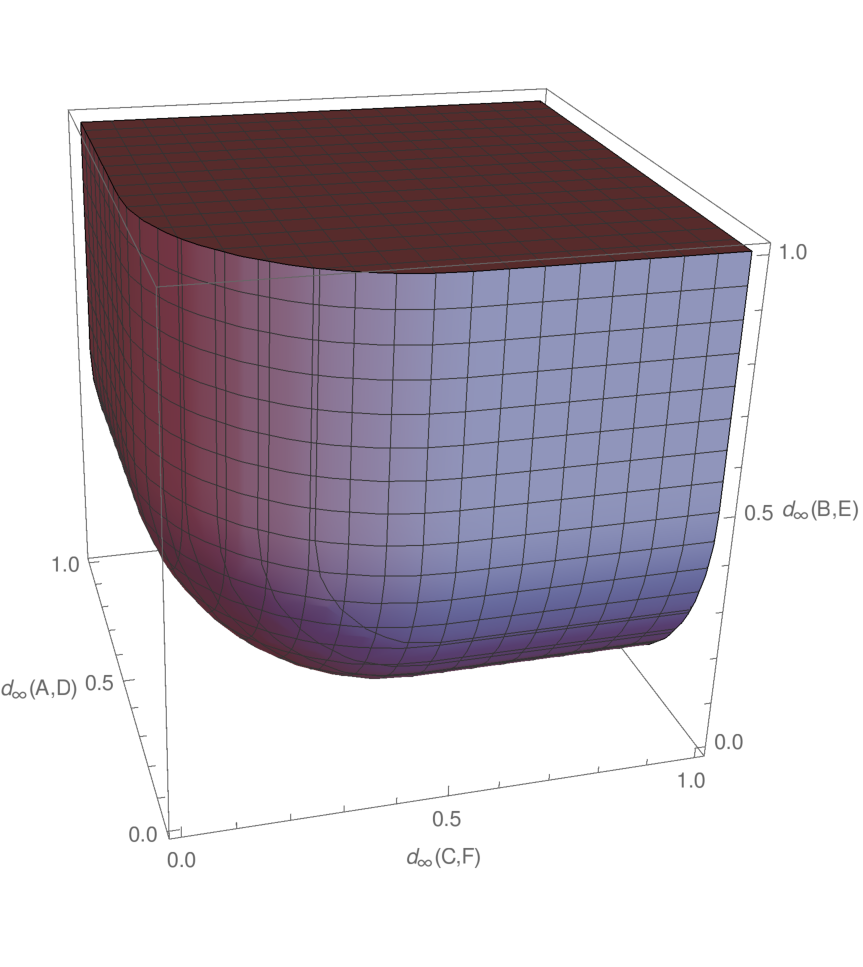
\includegraphics[width=0.35\textwidth]{ur1triple2.pdf}
  }
  \subfloat{
    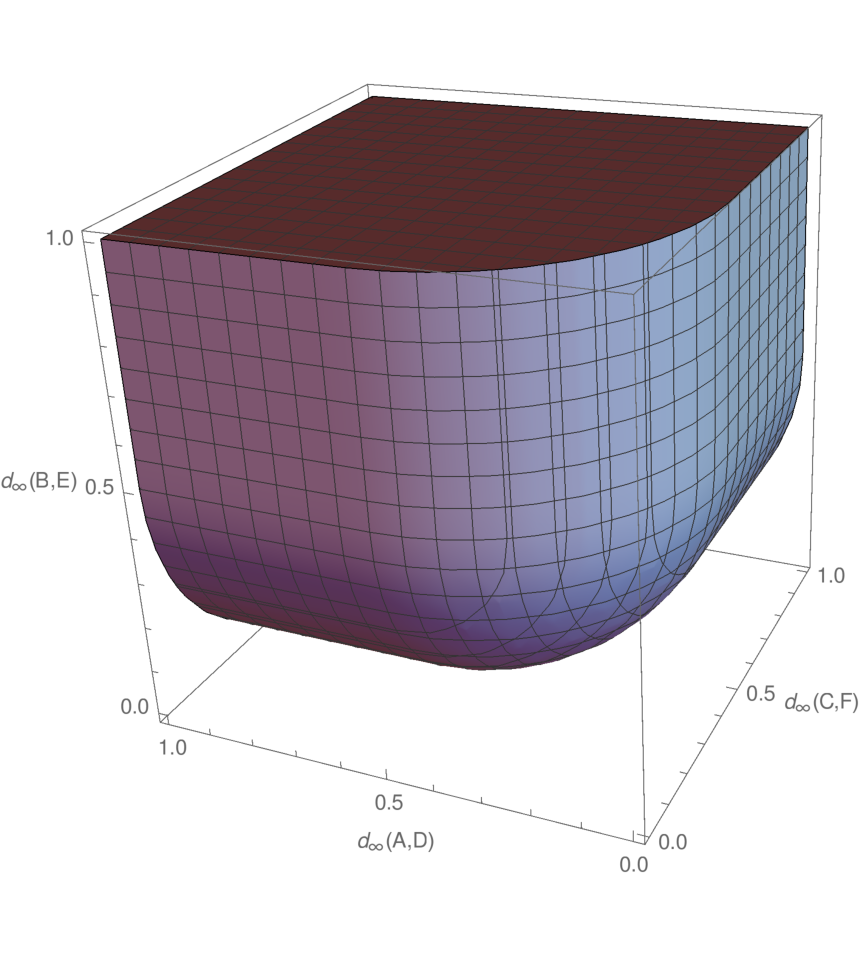
\includegraphics[width=0.35\textwidth]{ur2triple2.pdf}
  }\\
  \subfloat{
    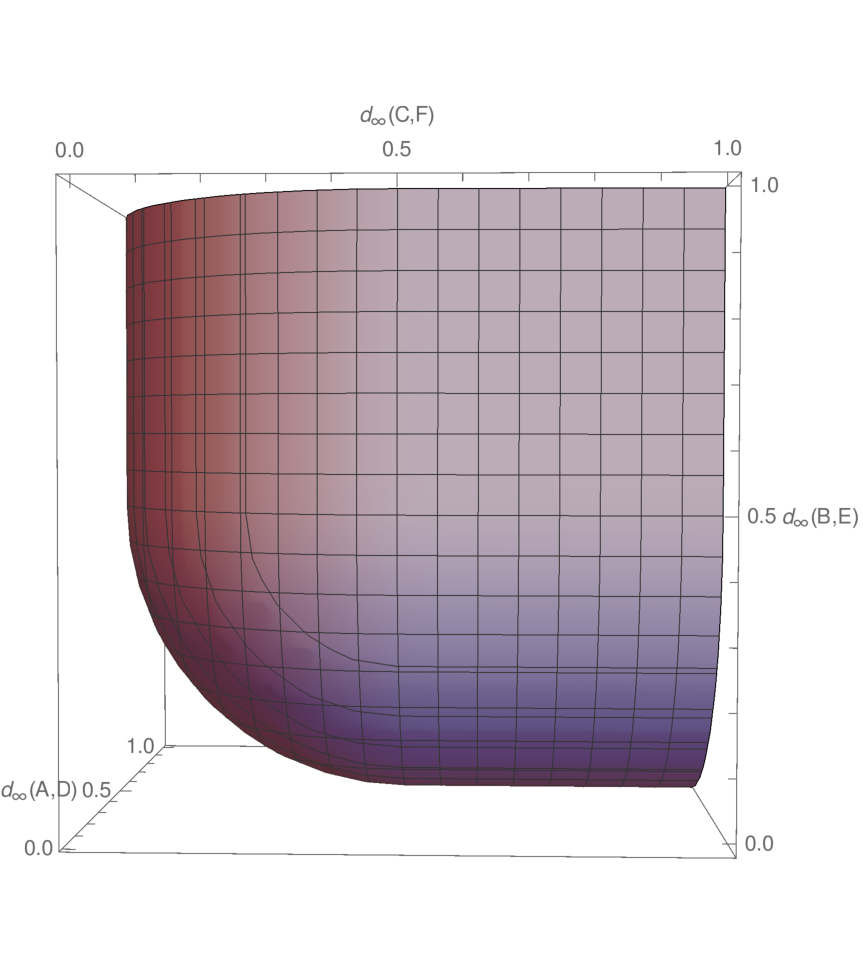
\includegraphics[width=0.35\textwidth]{ur3triple2.pdf}
  }
  \subfloat{
    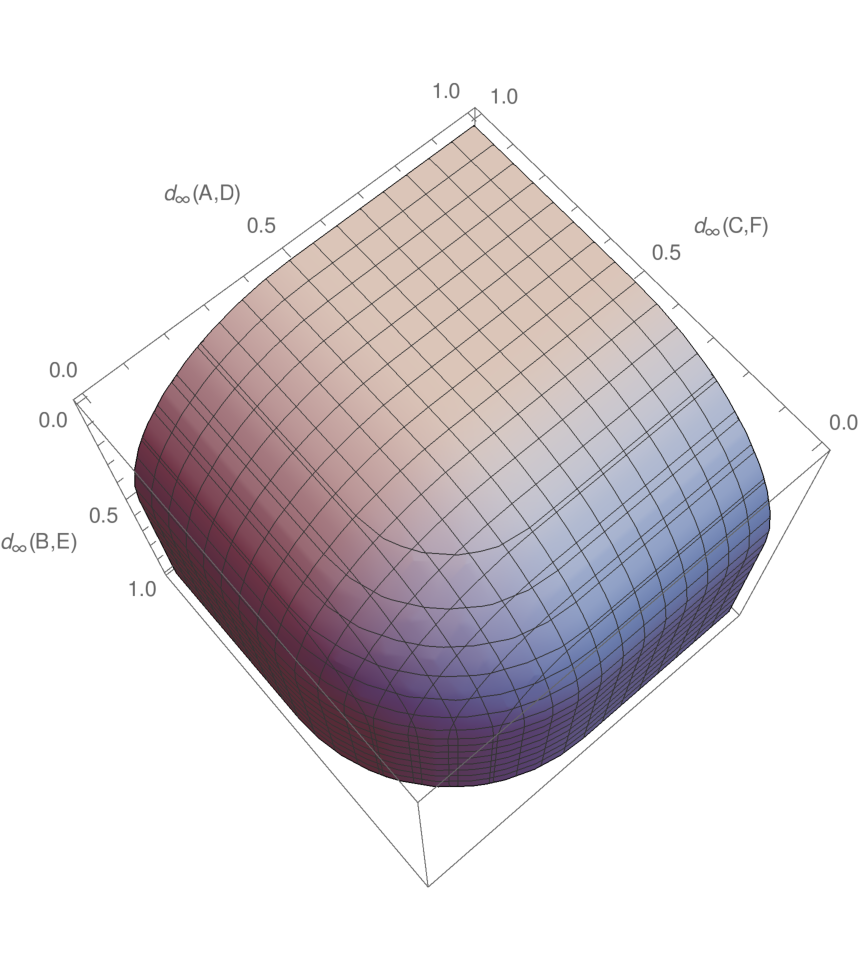
\includegraphics[width=0.35\textwidth]{ur4triple2.pdf}
  }
  \caption{Various views of the uncertainty region $S_\infty(\opa.\opb,\opc)$ covered by compatible approximations $\opd$, $\ope$ and $\opf$.}
\end{figure}

\section{The Fourier pair}
\label{sec:fourier-pair}
Let $\cyc[n] = \{0\hdots n-1\}$ denote the cyclic group of order $n$, equivalent to the set of natural numbers less than $n$, with the group operation addition modulo $n$, denoted $+$. Although this is only a field for $n$ prime, it will be useful to define multiplication, denoted by juxtaposition, as the usual multiplication of natural numbers modulo $n$. 

Let $\hcal$ be a Hilbert space of dimension $n\in\mathbb{N}$, $n \geq 2$, $\sbuild{\ket{g}}{g \in \cyc[n]}$ be an orthonormal set of vectors, hereafter called the \emph{computational basis} and let
\begin{align}
  \ket{f_h} &\defeq \sqrt{\frac{1}{n}}\sum_{g\in \cyc[n]} e^{\frac{2\pi i}{n} gh}\ket{g}, \quad h\in\cyc[n]\\
  \implies \ket{g} &= \sqrt{\frac{1}{n}}\sum_{h\in \cyc[n]} e^{-\frac{2\pi i}{n} gh} \ket{f_h}, \quad g\in\cyc[n]
\end{align}
be the well known \emph{Fourier basis}. It is easily verified that the $\ket{f_h}$ are an orthonormal basis for $\hcal$ and are \emph{mutually unbiased} with the computational basis. We define sharp observables for these bases
\begin{align}
  \opa&:\cyc[n] \to \posops[\hcal] & \opb&:\cyc[n] \to \posops[\hcal]\\
  \opa&:g\mapsto \ketbra{g}{g} & \opb&:h\mapsto \ketbra{f_h}{f_h}.
\end{align}
We can define unitary \emph{shift operators} for these bases
\begin{align}
  U_k \ket{g} &= \ket{g + k} & \forall g,k\in\cyc[n]\\
  V_q \ket{f_h} &= \ket{f_{h+q}}&\forall h,q\in\cyc[n],
\end{align}
and note that each form a unitary representation of the group $\cyc[n]$. Further, we have that
\begin{align}
  U_k &= \sum_{h\in\cyc[n]}e^{-\frac{2\pi i}{n} k h}\ketbra{f_h}{f_h} = \sum_{h\in\cyc[n]}e^{-\frac{2\pi i}{n} k h}\,\opb(h)\\
  V_q &= \sum_{g\in\cyc[n]}e^{\frac{2\pi i}{n} q g}\ketbra{g}{g} = \sum_{g\in\cyc[n]}e^{\frac{2\pi i}{n} q g}\,\opa(g).
\end{align}
% \begin{align}
%   U_k \ket{f_h} &= e^{-\frac{2\pi i}{n}kh} \ket{f_h} \implies U_k \ketbra{f_h}{f_h} U_k^\dagger = \ketbra{f_h}{f_h}\\
%   V_q \ket{g} &= e^{\frac{2\pi i}{n}gq} \ket{g}  \implies V_q \ketbra{g}{g} V_q^\dagger = \ketbra{g}{g}
% \end{align}
It is easy to verify the commutation relations
\begin{align}
  U_k V_q  &= e^{\frac{2\pi i}{n} kq}  V_q U_k,
\end{align}
by, for example, applying the operator on each side of the equality to the states in the Fourier basis. Therefore
\begin{align}
  U_k V_q \rho\, V_q^\dagger U^\dagger_k = V_q U_k \rho\,  U^\dagger_k V_q^\dagger, \quad \forall \rho\in\saops[\hcal].
\end{align}
We therefore consider the linear maps
\begin{align}
  R_{k,q}&:\saops[\hcal]\to \saops[\hcal]\\
  R_{k,q}&:\rho \mapsto U_k V_q \rho\, V^\dagger_q U^\dagger_k =  V_q U_k  \rho\,  U^\dagger_k V^\dagger_q,
\end{align}
and note that they form a representation of the direct product group $\cyc[n]\times\cyc[n]$, with the group operation given by operator composition
\begin{align}
  R_{k,q} \circ R_{l,r} = R_{k+l, p+r}, \quad \forall k,l,q,r\in \cyc[n].
\end{align}
These maps act on the effects of the target observables correctly
\begin{align}
  R_{k,q}\left[\ketbra{g}{g}\right] &=  \ketbra{g+k}{g+k}\\
  R_{k,q}\left[\ketbra{f_h}{f_h}\right] &=  \ketbra{f_{h+q}}{f_{h+q}}.
\end{align}
Therefore we can apply the theorems of section \ref{sec:invariant-mean} to establish that the covariant joint observables are optimal with respect to the $d_p$ distance measures.

\subsection{Commutivity} 
There is a one-to-one relation between covariant joint observables $\opj:\cyc[n]\times\cyc[n]\to\posops[\hcal]$ and trace one positive operators on $\hcal$ given by 
\begin{align}
  \opj:(k,q)\mapsto \frac{1}{n}R_{k,q}\left[\tau\right].
\end{align}
All covariant, $\cyc[n]\times\cyc[n]$ valued observable are obtained in this way, for some trace $1$ positive $\tau$, as we can take $\tau = n\opj(0,0)$, and all trace $1$ positive operators give rise to some covariant, $\cyc[n]\times\cyc[n]$ valued observable. We can write down the margins of such an observable
\begin{align}
  \opc&:\cyc[n] \to \posops[\hcal] & \opd&:\cyc[n] \to \posops[\hcal]\\
  \opc&:g\mapsto \sum_h \opj(g,h) = \frac{1}{n}\sum_h R_{g,h}\left[\tau\right] &  \opd&:h\mapsto \sum_g \opj(g,h) = \frac{1}{n}\sum_g R_{g,h}\left[\tau\right].
  \label{eqn:write-down-margins}
\end{align}
% First note the identity
% \begin{align}
%   \sum_{r}e^{-\frac{2\pi i}{n}rl}\ket{f_{r+h}} &= V_h \sum_{r}e^{-\frac{2\pi i}{n}rl}\ket{f_r} \\
%                                                &= V_h \sqrt{n}\ket{l} \\
%                                                &=  \sqrt{n}e^{\frac{2\pi i}{n} lh}\ket{l}
% \end{align}
We can show that each $\opc(k)$ commutes with each $V_q$
\begin{align}
  \opc(g) &= \sum_h \opj(g,h)\\
          &= \sum_h \opj(g, h+q)\\
          &= \sum_h R_{0,q}[\opj(g,h)]\\
          &= V_q \opc(g) V_q^*\\
  \implies \opc(g) V_q &= V_q \opc(g), \quad \forall g,q\in \cyc[n].
\end{align}
A similar calculation gives
\begin{align}
  \opd(h) U_k = U_k \opd(h), \quad \forall h,k\in \cyc[n].
\end{align}
Indeed an explicit calculation gives
% \begin{align}
%   \opc(0) &= \sum_h \opj(0,h)\\
%           &= \frac{1}{n}\sum_h R_{0,h}\left[\tau\right]\\
%           &= \frac{1}{n}\sum_h V_h \tau V_h^\dagger \\
%           &= \frac{1}{n}\sum_{h} \sum_{q,r} \ketbra{f_{q+h}}{f_q} \tau \ketbra{f_r}{f_{r+h}} \\
%           &= \frac{1}{n} \sum_{h}\sum_{q,r} \bra{f_{q+h}} \tau \ket{f_{r+h}} \ketbra{f_{q}}{f_{r}} \\
%           &= \frac{1}{n^2} \sum_{k,l} \ketbra{k}{l} \sum_{h}\sum_{q,r} \bra{f_{q+h}} \tau \ket{f_{r+h}}  e^{\frac{2\pi i}{n}(qk- rl)}\\
%           &= \frac{1}{n^2} \sum_{k,l} \ketbra{k}{l} \sum_{h} \left(\sum_{q}\bra{f_{q+h}}e^{\frac{2\pi i}{n}qk}\right) \tau \left(\sum_{r}e^{-\frac{2\pi i}{n}rl}\ket{f_{r+h}}\right)  \\
%           &= \frac{1}{n} \sum_{k,l} \ketbra{k}{l} \sum_{h} e^{-\frac{2\pi i}{n}kh }\bra{k} \tau e^{\frac{2\pi i}{n} lh}\ket{l}\\
%           &= \frac{1}{n} \sum_{k,l} \ketbra{k}{l} \bra{k} \tau \ket{l} \sum_{h}e^{\frac{2\pi i}{n}h(l-k) }\\
%           &= \sum_{k,l} \ketbra{k}{l} \bra{k} \tau \ket{l} \delta_{k,l}\\
%           &= \sum_{k} \ketbra{k}{k} \bra{k} \tau \ket{k},
% \end{align}

% where we use $\delta$ for the Kronecker delta. Since $\opc(g) = U_g \opc(0) U_g^\dagger$ this implies
\begin{align}
  \opc(g) &= \sum_{k} \ketbra{k+g}{k+g} \bra{k} \tau \ket{k}\\
  \opd(h) &= \sum_{q} \ketbra{f_{q+h}}{f_{q+h}} \bra{f_{q}} \tau \ket{f_{q}}.
\end{align}
\subsection{Computing the sup-norm}
The simultaneous diagonalisability of $\opa$ and $\opc$ allows us to compute $d_\infty(\opa,\opc)$ explicitly. Without loss of generality let
\begin{align}
  \opc(0) = \sum_{k\in\cyc[n]} c_k \ketbra{k}{k}
\end{align}
for $c_k\in \left[0,1\right]$, and $\sum_k c_k = 1$. Then
\begin{align}
  d_\infty(\opa,\opc) &= \sup_\rho \max_{g} \abs{\tr{\rho\left[\opa(g) - \opc(g)\right]}} \\
                      &=  \sup_\rho \max_g \abs{\tr{\rho\left[\ketbra{g}{g} - U_g\sum_{k\in\cyc[n]}c_k\ketbra{k}{k} U_g^\dagger\right]}} \\
                      &=  \sup_\rho \max_g \abs{\tr{\rho U_g\left[\ketbra{0}{0} - \sum_{k\in\cyc[n]}c_k\ketbra{k}{k} \right]U_g^\dagger}} \\
                      &=  \sup_\rho \max_g \abs{\tr{U_g^\dagger \rho U_g\left[\ketbra{0}{0} - \sum_{k\in\cyc[n]}c_k\ketbra{k}{k} \right]}} \\
                      &=  \sup_\rho \abs{\tr{\rho \left[\ketbra{0}{0} - \sum_{k\in\cyc[n]}c_k\ketbra{k}{k} \right]}} \\
                      &=  \max\{1-c_0, c_1, \hdots, c_{n-1}\}.
\end{align}
Now note that
\begin{align}
  \sum_{k\in\cyc[n]} c_k = 1 \implies \sum_{k\neq 0} c_k = 1-c_0
\end{align}
combined with $c_k \geq 0$ we see that
\begin{align}
  1-c_0 \geq c_k, \quad \forall k > 0,
\end{align}
so
\begin{align}
  \label{eqn:comp-constraint}
  d_\infty(\opa,\opc) = 1-c_0.
\end{align}
Similarly, if
\begin{align}
  \opd(0) = \sum_{r\in\cyc[n]} d_r \ketbra{f_r}{f_r},
\end{align}
then
\begin{align}
  \label{eqn:four-constraint}
  d_\infty(\opb,\opd) = 1-d_0.
\end{align}
\subsection{Semidefinite program}
We can use relations \eqref{eqn:comp-constraint} and \eqref{eqn:four-constraint}, along with \eqref{eqn:write-down-margins} to put constraints on the operator $\tau$ we used to define the joint
\begin{align}
  \sum_h \opj(g,h) &= \opc(g) = U_g \opc(0) U_g^\dagger\\
  \frac{1}{n} \sum_h U_gV_h \tau V_h^\dagger U_g^\dagger &= U_g \opc(0) U_g^\dagger\\
  \iff \frac{1}{n} \sum_h V_h \tau V_h^\dagger  &=  \opc(0)  \\
  \frac{1}{n} \sum_g U_g \tau U_g^\dagger  &=  \opd(0).
\end{align}
Computing matrix elements gives
\begin{align}
  \bra{k} \opc(0) \ket{l} = \frac{1}{n} \sum_h \bra{k} V_h \tau V_h^\dagger \ket{l} &= \frac{1}{n} \sum_h \bra{k} V_h^\dagger \tau V_h \ket{l} \\
                                                                          &= \frac{1}{n} \sum_h \bra{k}\tau \ket{l} e^{\frac{2\pi i}{n} h(l-k)}\\
                                                                          &= \bra{k}\tau \ket{l} \delta_{k,l}\\
  \bra{f_r} \opd(0) \ket{f_s} &= \bra{f_r}\tau \ket{f_s} \delta_{r,s}.
\end{align}
Given that the only matrix elements that affect the uncertainties are the $(0,0)$ matrix element of $\opc(0)$ and the $(f_0, f_0)$ matrix element of $\opd(0)$ the relevant constraints are
\begin{align}
  \bra{0}\tau\ket{0} &= 1 - d_\infty(\opa,\opc)\\
  \sum_{k,l} \bra{k}\tau\ket{l} &=  n(1- d_\infty(\opb,\opd)).
\end{align}
If we set 
\begin{align}
  A_n &= \sum_{k,l} \ketbra{k}{l}
\end{align}
then computing the lower boundary of the uncertainty region is equivalent to the following semidefinite program, for each $d_a\in [0,1]$
\begin{equation}
  \begin{aligned}
    & \underset{X}{\text{maximise}}
    & & p = \tr{A_n X} \\
    & \text{subject to}
    & \tr{\ketbra{0}{0} X} &= 1-d_a, \\
    &&  \tr{\opi_n  X} &= 1, \\
    && X &\geq 0.
  \end{aligned}
  \label{eqn:semidefinite-program}
\end{equation}
We can impose the equality constraints in \eqref{eqn:semidefinite-program}, by means of the linear map
\begin{align}
  \mathcal{M}&: \saops[\hcal] \to M_2(\mathbb{C})\\
  \mathcal{M}&:X \mapsto \begin{pmatrix}\tr{\ketbra{0}{0} X} & 0 \\ 0 & \tr{X}\end{pmatrix},
\end{align}
where $M_2(\mathbb{C})$ is the set of $2$ by $2$ matrices over the field $\mathbb{C}$. If
\begin{align}
  B = \begin{pmatrix}1-d_a & 0 \\ 0 & 1\end{pmatrix}
\end{align}
then the equality constraints are
\begin{align}
  \mathcal{M}(X) = B
\end{align}
We can compute the dual of $\mathcal{M}$ directly from the defining relation
\begin{align}
  \tr{\mathcal{M}^*(Y) X} &= \tr{Y \mathcal{M}(X)}\\
                          &= Y_{00} \tr{\ketbra{0}{0}X} + Y_{11} \tr{\opi_n X} \\
  \mathcal{M}^*\left(\begin{pmatrix}Y_{00} & Y_{01} \\ Y_{10} & Y_{11}\end{pmatrix}\right) &= Y_{00} \ketbra{0}{0} + Y_{11}\opi_n.
\end{align}
The dual problem to \eqref{eqn:semidefinite-program} is then given by
\begin{equation}
  \begin{aligned}
    & \underset{Y}{\text{minimise}}
    & d &= \tr{B Y} \\
    & \text{subject to}
    & \mathcal{M}^*(Y) &\geq A_n\\
    && Y &\in M_2(\mathbb{C}).
  \end{aligned}
  \label{eqn:semidefinite-program-dual}
\end{equation}
Alternatively 
\begin{equation}
  \begin{aligned}
    & \underset{y_0, y_1\in\mathbb{R}}{\text{minimise}}
    & d &= (1-d_a)y_0 + y_1 \\
    & \text{subject to}
    & 0&\leq y_0 \ketbra{0}{0} + y_1 \sum_k \ketbra{k}{k} - \sum_{k,l} \ketbra{k}{l} = Z.
  \end{aligned}
\end{equation}
It is easy to see that we have \emph{strong duality} for these problems, since we can always choose $y_1$ large enough that $Z > 0$, by the Slater condition\cite{rtr-conv-anal-book} we therefore know that wherever the solution $d$ to the dual problem is finite we have that $\inf d=\sup p$.

% We can also choose $X = (1-d_a)\ketbra{0}{0} + \frac{d_a}{n-1}\left(\sum_{k>0} \ketbra{k}{k}\right) > 0$, for $d_a\in(0,1)$ as a strictly feasible solution to the primal problem. Thus the optimal set is non-empty, and the optimum finite in this range.

Henceforth we mix operators interchangeably with their matrices in the computational basis. Define the \emph{characteristic polynomial} function for each $n\in\mathbb{N}$
\begin{align}
  \chi_n:M_n(\mathbb{C})\times \mathbb{R} &\to \mathbb{R}\\
  \chi_n(X, x) &= \det(x\opi_n - X).
\end{align}
We can compute the characteristic polynomial of the matrix $Z$
\begin{align}
  \chi_n(Z,x) &= \det\left(x\opi_n -Z\right)\\
              &=\det\left((x-y_1)\opi_n - y_0\ketbra{0}{0} + A_n\right)\\
              &=\det\left((x-y_1)\opi_n + A_n\right) -y_0 \bra{0}\adj{(x-y_1)\opi_n + A_n} \ket{0}\\
              &=\det\left((x-y_1)\opi_n + A_n\right) -y_0 \det\left((x-y_1)\opi_{n-1} + A_{n-1}\right)\\
              &=(-1)^n \det\left((y_1-x)\opi_n - A_n\right) -(-1)^{n-1} y_0 \det\left((y_1-x)\opi_{n-1} - A_{n-1}\right)\\
              &=(-1)^n \chi_n(A_n,y_1-x)  + (-1)^{n} y_0 \chi_{n-1}(A_{n-1}, y_1-x)\\
              &= (-1)^n\left[(x-y_1-n)(x-y_1)^{n-1} +y_0(x-y_1-n+1)(x-y_1)^{n-2}\right]\\
              &= (-1)^n(x-y_1)^{n-2}\left[(x-y_1-n)(x-y_1) -y_0(x-y_1-n+1)\right]\\
              &= (-1)^n(x-y_1)^{n-2}\left[x^2 + x(n-y_0 -2y_1) + \left(y_1^2 + y_1(y_0-n) + y_0(1-n)\right)\right]
                \label{eqn:char-poly}
\end{align}
where $\operatorname{adj}$ denotes the adjudicate matrix, and we have employed the classical matrix determinant lemma, as well as the fact that
\begin{align}
  \chi_n(A_n,x) = (x-n)x^{n-1},
\end{align}
for $A_n$ the $n$ by $n$ matrix of ones \cite{matrix-analysis}.
We are seeking constraints on $y_0$ and $y_1$ which are necessary and sufficient for all of the roots of $x\mapsto \chi_n(Z,x)$ to be non-negative, we can read off from \eqref{eqn:char-poly} that $y_1 \geq 0$. We now need to examine the roots of 
\begin{align}
  x\mapsto x^2 + x(n-y_0 -2y_1) + \left(y_1^2 + y_1(y_0-n) + y_0(1-n)\right),
\end{align}
the quadratic formula gives
\begin{align}
  x^\pm = \frac{1}{2}\left(y_0 +2y_1 -n \pm \sqrt{(y_0 + 2y_1 -n)^2 - 4(y_1^2 + y_1(y_0-n) + y_0(1-n))} \right),
\end{align}
note that the roots are automatically real, as our matrices are self-adjoint. The $x^\pm$ are both non-negative if, and only if
\begin{align}
  \sqrt{(y_0 + 2y_1 -n)^2 - 4(y_1^2 + y_1(y_0-n) + y_0(1-n))} \leq y_0 +2y_1 -n,
\end{align}
which is satisfied if and only if
\begin{align}
  0&\leq y_0 +2y_1 -n,
     \label{eqn:y1-consraint-1}
\end{align}
and
\begin{align}
 0&\leq y_1^2 + y_1(y_0-n) + y_0(1-n),
    \label{eqn:y1-constraint-2}
\end{align}
are both satisfied. The solutions of
\begin{align}
  y_1^2 + y_1(y_0-n) + y_0(1-n) = 0
\end{align}
are
\begin{align}
  y_1^\pm = \frac{1}{2}\left(n-y_0 \pm \sqrt{(n-y_0)^2 - 4y_0(1-n)}\right).
\end{align}
It is easy to show that the radicant is positive. The constraint in \eqref{eqn:y1-constraint-2} is therefore satisfied if, and only if
\begin{align}
  y_1 \geq \frac{1}{2}\left(n-y_0 + \sqrt{(n-y_0)^2 + 4y_0(n-1)}\right)
\end{align}
or
\begin{align}
  y_1 \leq \frac{1}{2}\left(n-y_0 - \sqrt{(n-y_0)^2 + 4y_0(n-1)}\right)
\end{align}
Rewriting \eqref{eqn:y1-consraint-1} we see we need
\begin{align}
  y_1 \geq \frac{1}{2}\left(n-y_0\right),
\end{align}
therefore all of the constraints are satisfied if, and only if
\begin{align}
  y_1 \geq \frac{1}{2}\left(n-y_0 + \sqrt{(n-y_0)^2 + 4y_0(n-1)}\right),
\end{align}
since the quantity on the right hand side is always positive. Recall that we are attempting to minimise the quantity
\begin{align}
  d &= (1-d_a)y_0 + y_1,
\end{align}
subject to the positivity constraints. We therefore choose
\begin{align}
  y_1 &= \frac{1}{2}\left(n-y_0 + \sqrt{(n-y_0)^2 + 4y_0(n-1)}\right)\\
  \implies d &= \left(\frac{1}{2} - d_a\right)y_0 + \frac{1}{2}\left(n+\sqrt{(n-y_0)^2 + 4y_0(n-1)}\right),
\end{align}
differentiating, we find that $d$ is minimised where
\begin{align}
  y_0 = 2-n - \abs{1-2d_a}\sqrt{\frac{n-1}{d_a(1-d_a)}},
\end{align}
and that at this point 
\begin{align}
  d &= 1 + d_a(n-2) + 2\sqrt{d_a(1-d_a)(n-1)}\\
  \implies d_b^{\text{min}} &= 1- \frac{d}{n}\\
    &= 1 -  \frac{1}{n}\left(1 + d_a(n-2) + 2\sqrt{d_a(1-d_a)(n-1)}\right).
\end{align}
We note that this is a section of the ellipse with defining equation
\begin{align}
0 = n^2d_a^2 + n^2 d_b^2 + 2n(n-2)d_ad_b + 2n(1-n)d_a + 2n(1-n)d_b  + (n-1)^2,
  \label{eqn:ellipse-defining-equation}
\end{align}
which has center $\left(\frac{1}{2}, \frac{1}{2}\right)$, and touches the coordinate axes at the points $\left(0, 1-\frac{1}{n}\right)$ and $\left(1-\frac{1}{n}, 0\right)$. The major axis of the ellipse has angle $\frac{\pi}{4}$ with each coordinate axis, as it must by symmetry.

\begin{figure}
  \centering
  \begin{subfigure}[t]{0.4\textwidth}
    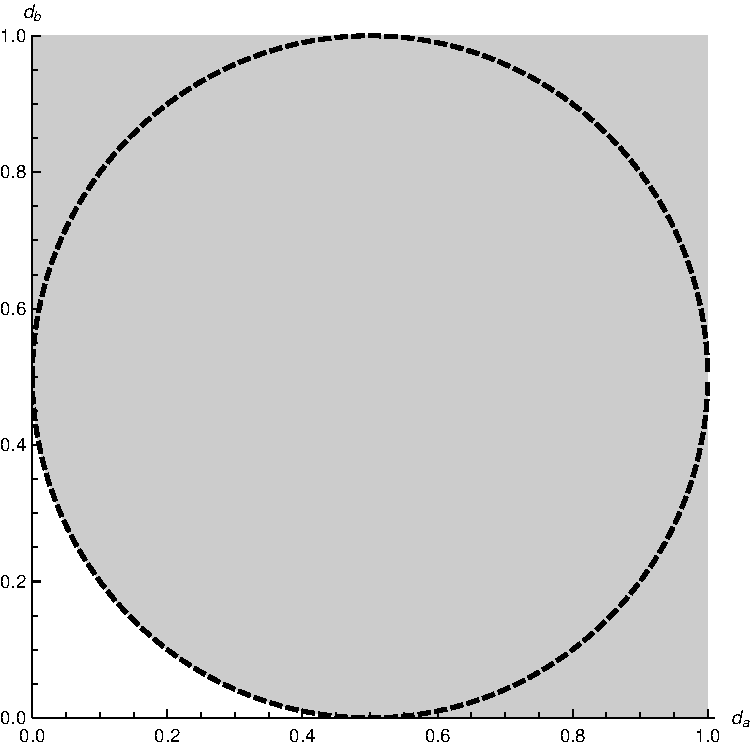
\includegraphics[width=\textwidth]{fourier-ur-2}
  \end{subfigure}\quad
  \begin{subfigure}[t]{0.4\textwidth}
    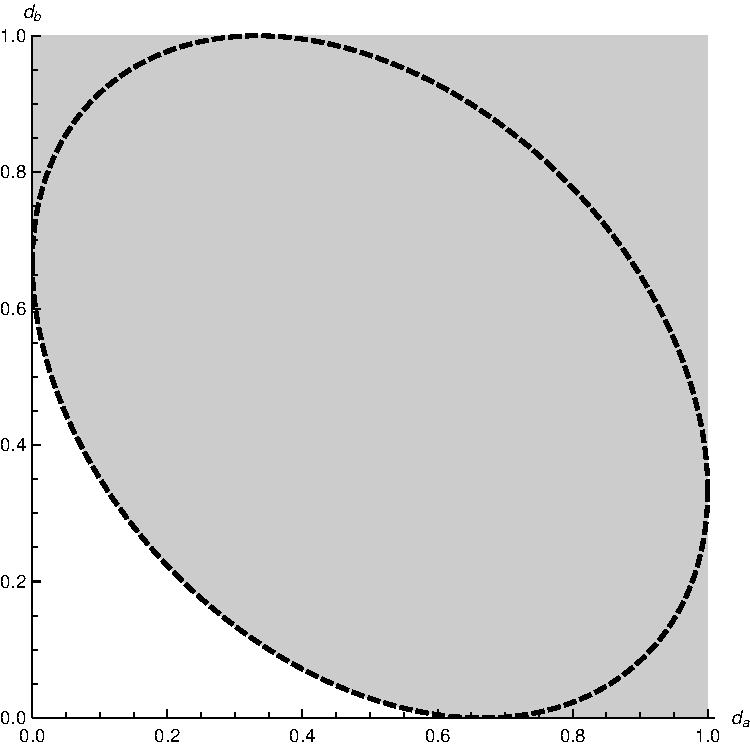
\includegraphics[width=\textwidth]{fourier-ur-3}
  \end{subfigure}\\
  \begin{subfigure}[t]{0.4\textwidth}
    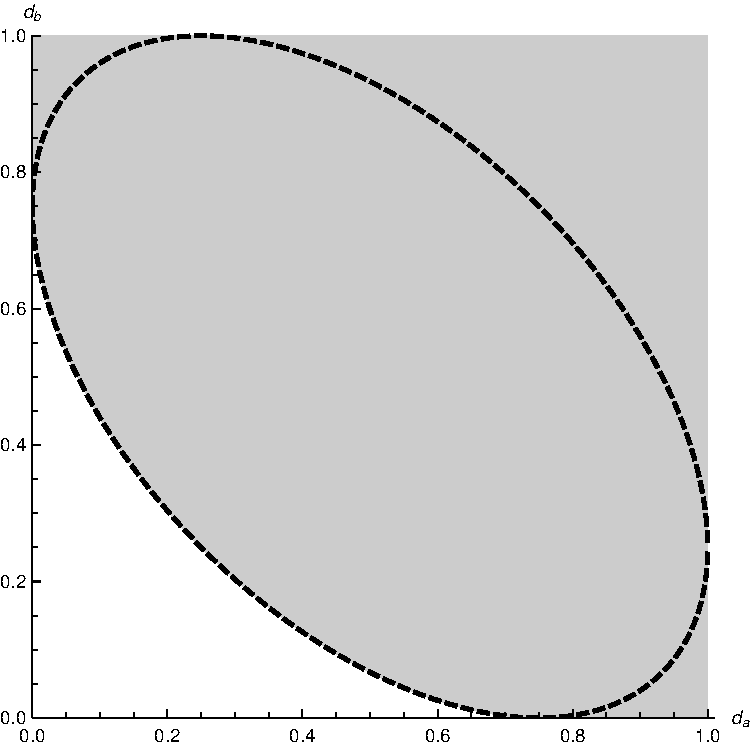
\includegraphics[width=\textwidth]{fourier-ur-4}
  \end{subfigure}\quad
  \begin{subfigure}[t]{0.4\textwidth}
    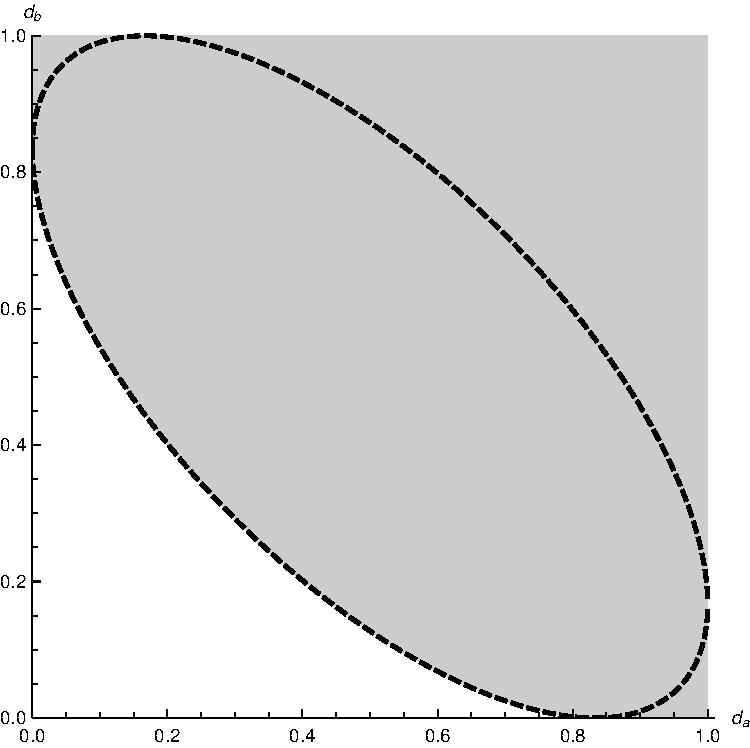
\includegraphics[width=\textwidth]{fourier-ur-6}
  \end{subfigure}\\
  \begin{subfigure}[t]{0.4\textwidth}
    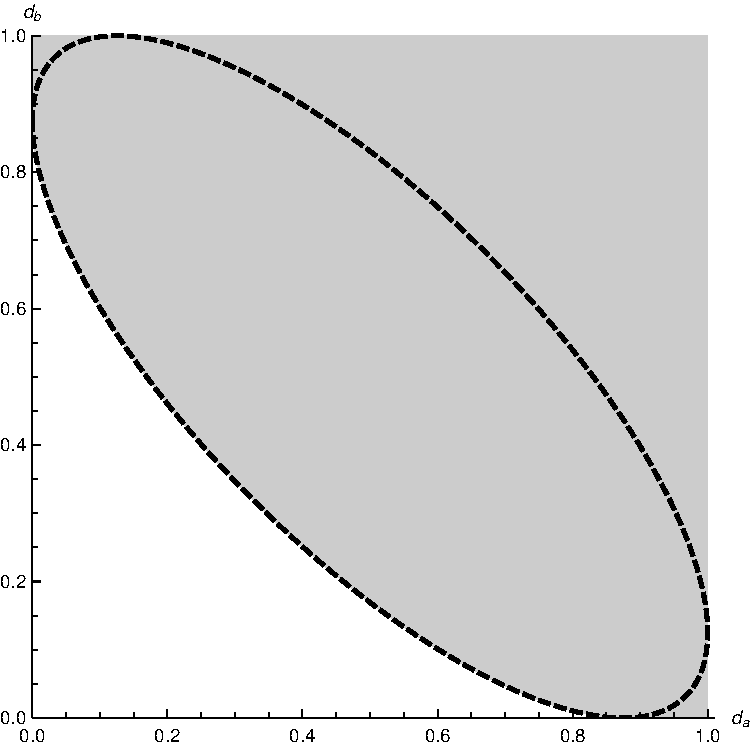
\includegraphics[width=\textwidth]{fourier-ur-8}
  \end{subfigure}\quad
  \begin{subfigure}[t]{0.4\textwidth}
    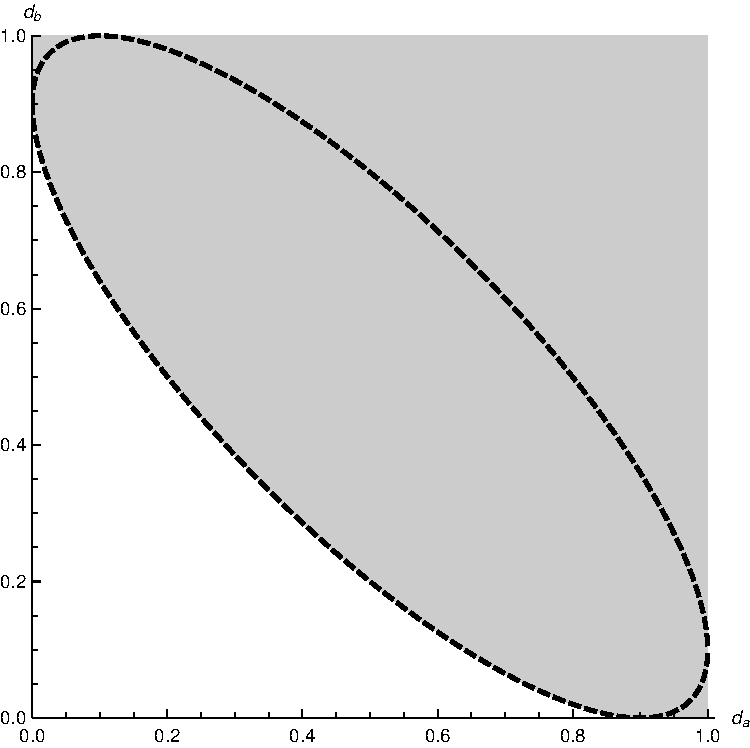
\includegraphics[width=\textwidth]{fourier-ur-10}
  \end{subfigure}\\
  \caption{The measurement uncertainty region for quantum Fourier pair observables in several dimensions.}
\end{figure}

% \begin{figure}
%   \begin{center}
%     \subfloat[$n=2$]{
%     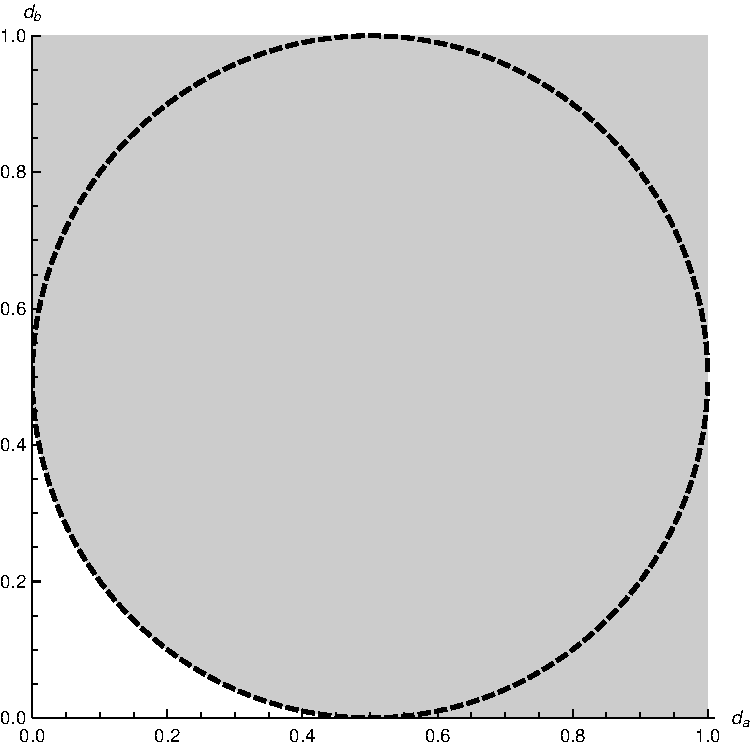
\includegraphics[width=0.4\textwidth]{fourier-ur-2}
%   } 
%   \subfloat[$n=3$]{
%     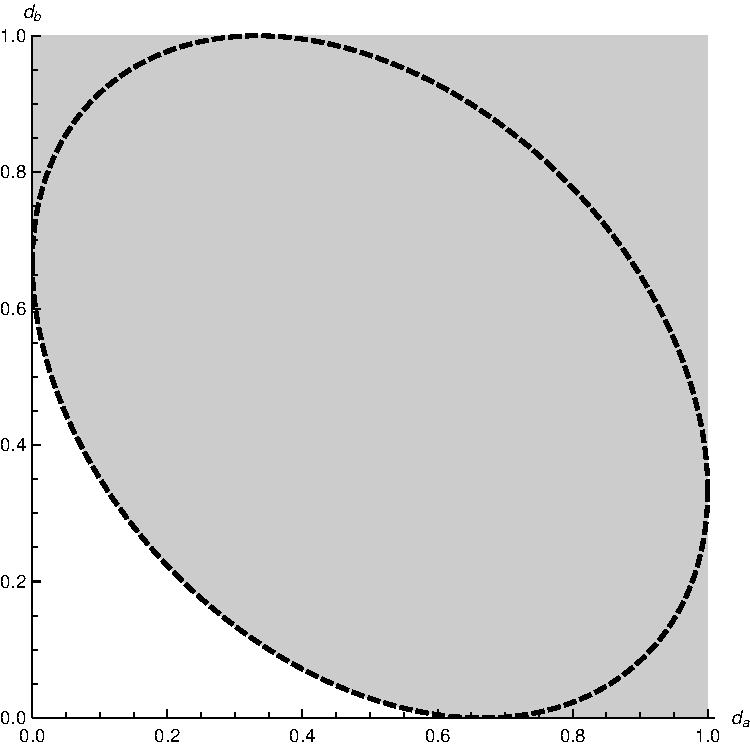
\includegraphics[width=0.4\textwidth]{fourier-ur-3}
%   } \\
%   \subfloat[$n=4$]{
%     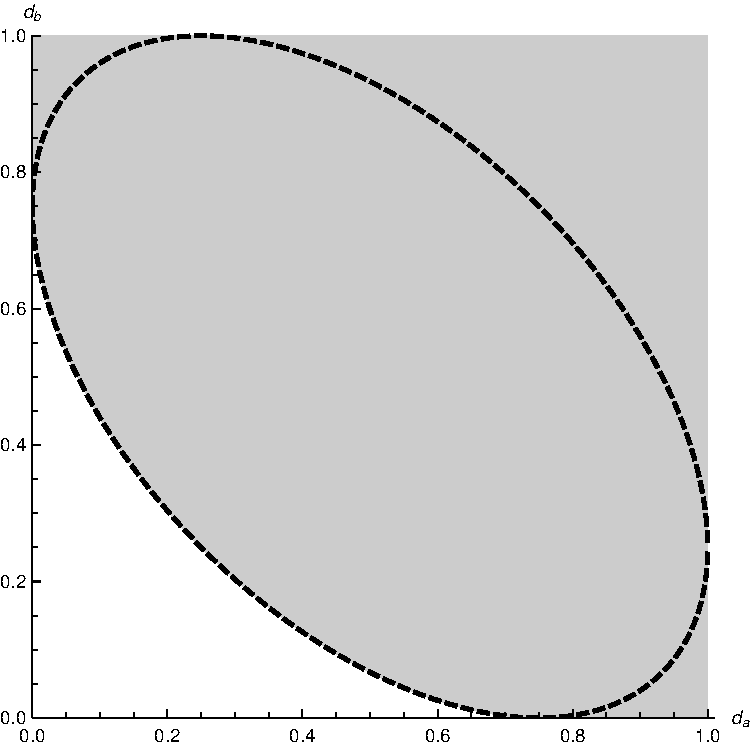
\includegraphics[width=0.4\textwidth]{fourier-ur-4}
%   } 
%   \subfloat[$n=6$]{
%     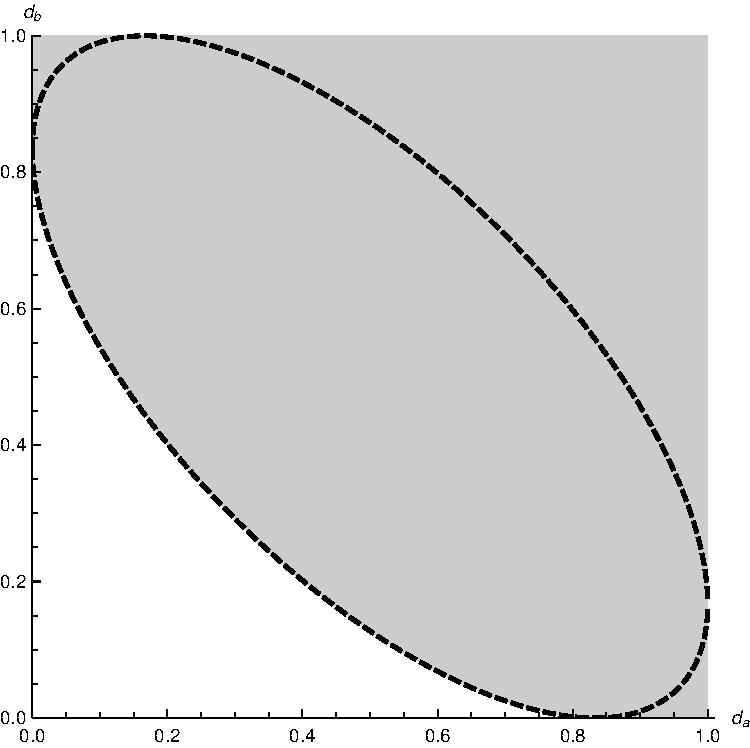
\includegraphics[width=0.4\textwidth]{fourier-ur-6}
%   } \\
%   \subfloat[$n=8$]{
%     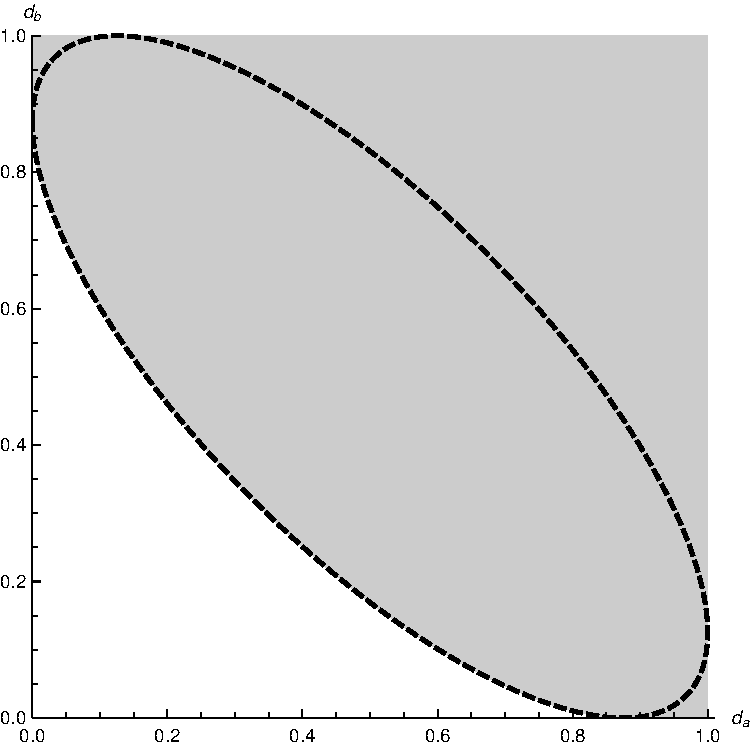
\includegraphics[width=0.4\textwidth]{fourier-ur-8}
%   } 
%   \subfloat[$n=10$]{
%     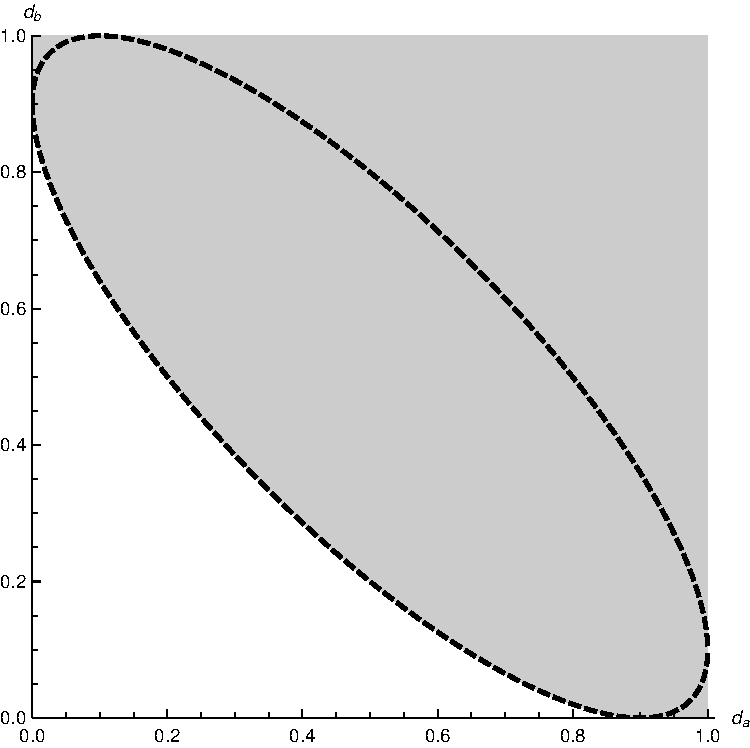
\includegraphics[width=0.4\textwidth]{fourier-ur-10}
%   } 
%   \caption{The complete and exact $d_\infty$ measurement uncertainty region for the Fourier pair in various dimension Hilbert spaces (shaded), with the ellipse \eqref{eqn:ellipse-defining-equation} (dashed line).}
% \end{center}
% \end{figure}



